\documentclass[12pt,a4paper]{report}
\usepackage[utf8]{inputenc}
\usepackage{amsmath}
\usepackage{algorithm}
\usepackage{algpseudocode}
\usepackage{amssymb}
\usepackage{graphicx}
\usepackage{geometry}
\usepackage[hidelinks]{hyperref}  % For clickable references
\usepackage[capitalise]{cleveref}  % For intelligent cross-referencing
\usepackage[english]{babel}

\usepackage{makecell}
\usepackage{caption}
\usepackage{array}
\usepackage{listings}
\usepackage{titlesec}
\usepackage{hyperref}
\hypersetup{
	colorlinks=true,
	linkcolor=black,
	filecolor=black,      
	urlcolor=cyan,
	citecolor=black
}

\graphicspath{{C:/Users/frabb/OneDrive - Cal Poly/Documents (Cloud)/0 CALPOLY/000Thesis/Chapters/Images/}}

\geometry{
	top=1in,
	bottom=1in,
	left=1.5in,
	right=1in
}

% Remove space before equations only
\makeatletter
\g@addto@macro\normalsize{%
	\setlength\abovedisplayskip{-10pt}
	\setlength\abovedisplayshortskip{-10pt}
}
\makeatother

% Updated list settings
\usepackage{enumitem}
\setlist[itemize]{nosep, leftmargin=*}
\setlist[enumerate]{nosep, leftmargin=*}

% Remove space before lists
\usepackage{etoolbox}
\BeforeBeginEnvironment{itemize}{\vspace{-\baselineskip}}
\BeforeBeginEnvironment{enumerate}{\vspace{-\baselineskip}}

\setlength{\parskip}{\baselineskip}
\titlespacing*{\section}{0pt}{0pt}{0pt}
\titlespacing*{\section}{0pt}{0pt}{-10pt}
\titlespacing*{\subsection}{0pt}{0pt}{-10pt}

\captionsetup[table]{skip=0pt}

\usepackage{xcolor}

\definecolor{codegreen}{rgb}{0,0.6,0}
\definecolor{codegray}{rgb}{0.5,0.5,0.5}
\definecolor{codepurple}{rgb}{0.58,0,0.82}
\definecolor{backcolour}{rgb}{0.95,0.95,0.92}

\lstdefinestyle{mystyle}{
	backgroundcolor=\color{backcolour},   
	commentstyle=\color{codegreen},
	keywordstyle=\color{magenta},
	numberstyle=\tiny\color{codegray},
	stringstyle=\color{codepurple},
	basicstyle=\ttfamily\footnotesize,
	breakatwhitespace=false,         
	breaklines=true,                 
	captionpos=b,                    
	keepspaces=true,                 
	numbers=left,                    
	numbersep=5pt,                  
	showspaces=false,                
	showstringspaces=false,
	showtabs=false,                  
	tabsize=2
}

\lstset{style=mystyle}

\title{Tutorial}
\author{Jakob Frabosilio}
\date{\today}
\setcounter{chapter}{2}
\begin{document}

\chapter{Acoustic Positioning System} \label{chap:3c}
The acoustic positioning system is the core of the iSBL-SF algorithm. In this system, an acoustic pulse is sent by a transmitter and recorded by receivers on the iSBL array. The time shift between the signals from each receiver is calculated, and these shifts are used to estimate the transmitter’s position relative to the iSBL array using an acoustic propagation model. Chapter \ref{chap:4c} describes how the orientation estimate of the platform is determined (and how dead reckoning is introduced), and Chapter \ref{chap:5c} details how Kalman filters are used to get the best position estimate by combining multiple data sources. This chapter describes only the acoustic positioning system, the central component of this thesis.

The first section in this chapter is dedicated to previous implementations of acoustic positioning systems, and how the iSBL approach differs from them. Next, the mechanical design of the receiver array is discussed. The electrical design of the acoustic positioning system, including the wiring diagram of the full iSBL array, is then detailed. The ultrasonic receivers receive their own section, where the design and manufacturing of the active band-pass filter PCB is explained. Then, the assembly of the full iSBL array is described, followed by the hardware and software design of the transmitter system. The final three sections are devoted to the software of the acoustic positioning system: how an acoustic pulse is detected and recorded, how the time shift between signals is calculated, and finally, how a position estimate is formed.

\section{Previous Works} \label{sec:3s1}
Acoustic positioning systems are not a new invention, and many different designs have been tested and implemented over the years. The rise of autonomous underwater vehicles has accelerated research into this field. In this section, the history of acoustic positioning systems is recounted, and the primary difference among these systems (the baseline length) is described. Lastly, similar implementations to this thesis are detailed.

\subsection{History of Acoustic Positioning Systems} \label{ssec:3s1s1}
The first known underwater acoustic positioning system was deployed in 1963, when a short baseline acoustic positioning system was used to guide the bathyscape \emph{Trieste 1} to the wreck of the US nuclear submarine USS \emph{Thresher}. The system barely worked, only guiding the \textit{Trieste} to the wreck once after ten unsuccessful attempts. The technology advanced as commercial applications became evident; oil and gas exploration in the 1970s was a primary driver for advancement. In 1998, a long baseline acoustic positioning system was used by a salvage company to navigate a debris field of a sunken WW2 Japanese submarine at 5240m deep. Current advancements in the field are primarily driven by the oil and gas industry, academic research, and defense industry applications \cite{apomab}.

\begin{figure}[htbp]
	\centering
	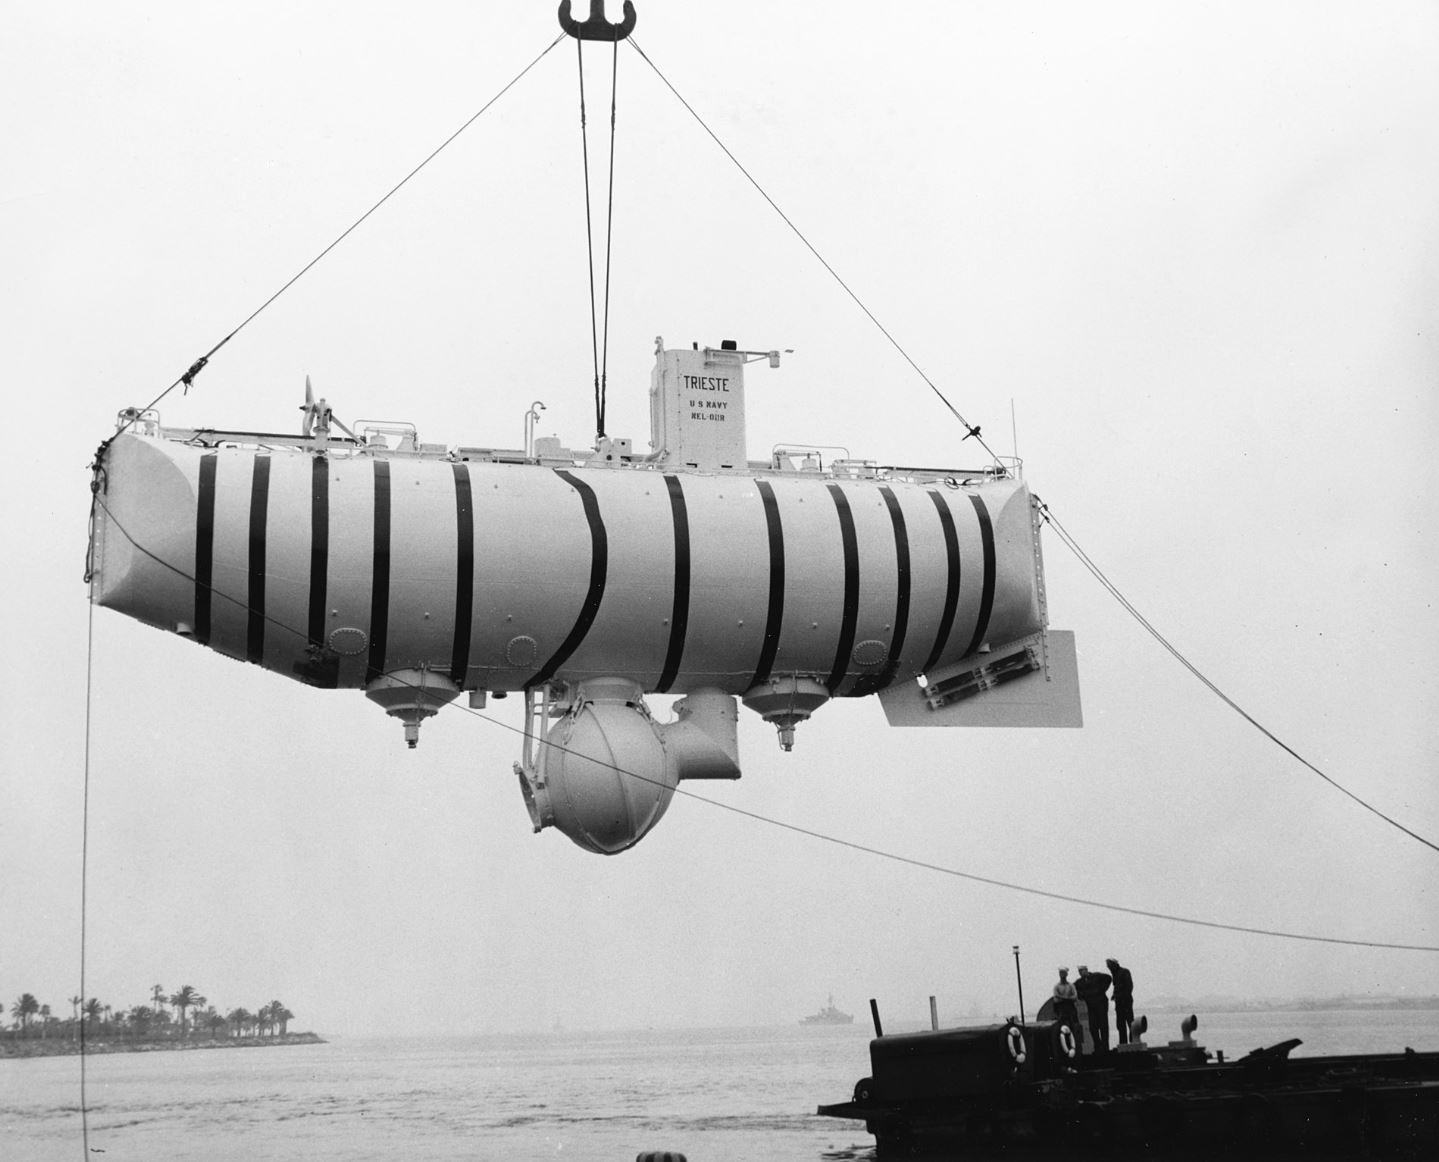
\includegraphics[width=0.5\textwidth]{trieste}
	\caption{Bathyscape \textit{Trieste 1}, which used the first short baseline acoustic positioning system to locate a nuclear submarine wreck \cite{apomab}}
	\label{fig:trieste}
\end{figure}

\subsection{Long, Short, Ultrashort, and Inverted Baselines} \label{ssec:3s1s2}
All acoustic positioning systems use the same core principle to function: sound waves propagate through a medium in a known and predictable way, and by sending acoustic waves from one or more transmitters to one or more receivers, the relative location between the transmitters and receivers can be determined. The primary way of differentiating underwater acoustic positioning systems is by their baseline, the spacing between receivers (or transmitters, depending on the system).

Long baseline (LBL) systems generally use multiple receivers spaced further than 100m apart in known, fixed locations; a transmitter is attached to the moving object whose position estimate is desired. LBL systems tend to have the best position accuracy when properly calibrated, but require many more resources and much more time to set up \cite{practicaloverview}. These systems are preferable when working in a single location for long periods of time and when sub-meter accuracy is desired \cite{apomab}. An additional benefit to LBL systems is that they tend to not require additional measurement equipment such as inertial measurement units or depth sensors, though additional equipment can improve accuracy. See Figure \ref{fig:lbldiagram} for an example of an LBL system.

\begin{figure}[htbp]
	\centering
	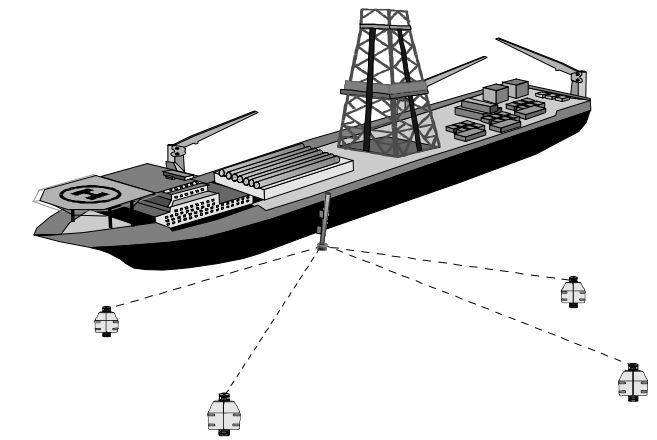
\includegraphics[width=0.5\textwidth]{lbldiagram}
	\caption{Long baseline acoustic positioning system diagram \cite{practicaloverview}}
	\label{fig:lbldiagram}
\end{figure}

Ultrashort baseline (USBL) systems generally use a single receiver module with multiple receiver elements spaced less than 10cm apart. These systems usually apply phase-differencing methods to compute the heading between the transmitter and receiver, with the receiver elements spaced less than one wavelength apart \cite{apomab}. These systems also tend to have low overall complexity and are contained in a single module; however, positional accuracy is less than LBL systems, and additional sensors (orientation sensors, vertical reference units) are required to obtain a position estimate \cite{practicaloverview}. See Figure \ref{fig:usbldiagram} for an example of a USBL system.

\begin{figure}[htbp]
	\centering
	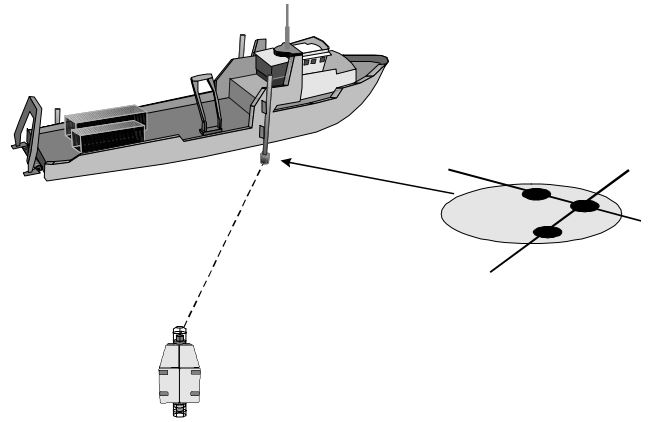
\includegraphics[width=0.5\textwidth]{usbldiagram}
	\caption{Ultrashort baseline acoustic positioning system diagram \cite{practicaloverview}}
	\label{fig:usbldiagram}
\end{figure}

Short baseline (SBL) systems are more broad and tend to encompass acoustic positioning systems whose baseline is greater than one wavelength (typically 1m - 100m) and whose receivers (or transmitters) are not fixed to the seafloor \cite{surveyurpn}. For example, the system of an ROV in the water equipped with a single transmitter and a boat on the surface of the water with receivers on each corner of the hull would be considered an SBL system. SBL systems tend to be a good middle-ground between LBL and USBL: they don’t require a fixed receiver array with massive baselines, but can produce position estimates that are close to LBL-level accuracy. These systems do require additional sensors like USBL systems do (orientation and depth), but the receiver array is generally attached to a vessel that already has these systems integrated. See Figure \ref{fig:sbldiagram} for an example of an SBL system.

\begin{figure}[htbp]
	\centering
	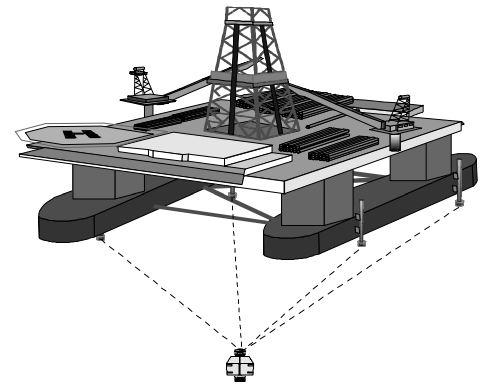
\includegraphics[width=0.5\textwidth]{sbldiagram}
	\caption{Short baseline acoustic positioning system diagram \cite{practicaloverview}}
	\label{fig:sbldiagram}
\end{figure}

Inverted acoustic positioning systems flip the location of the transmitter and receiver arrays. An inverted ultrashort baseline (iUSBL) places the transmitter on the surface of the water (generally on a research vessel or buoy with a known location) and the receiver module on an underwater vehicle - see Figure \ref{fig:iusblukf} for an example. Due to the small size of USBL system (with the receiver being similar in size to the transmitter), iUSBL systems are quite common, especially in autonomous underwater vehicles \cite{noveliusbl} \cite{passiveiusbl}.

\begin{figure}[htbp]
	\centering
	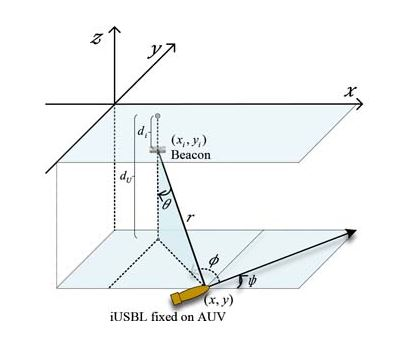
\includegraphics[width=0.6\textwidth]{iusblukf}
	\caption{Inverted ultrashort baseline system example \cite{iusblukf}}
	\label{fig:iusblukf}
\end{figure}

Inverted LBL and SBL systems are much more rare; only one paper espouses an iLBL system, whose diagram is shown in Figure \ref{fig:ilbl} below. Throughout the research for this thesis, no known papers have been written about iSBL systems - most systems that would use a receiver array on an underwater vehicle tend to space the receivers less than a baseline apart, or otherwise call themselves iUSBL systems.

\begin{figure}[htbp]
	\centering
	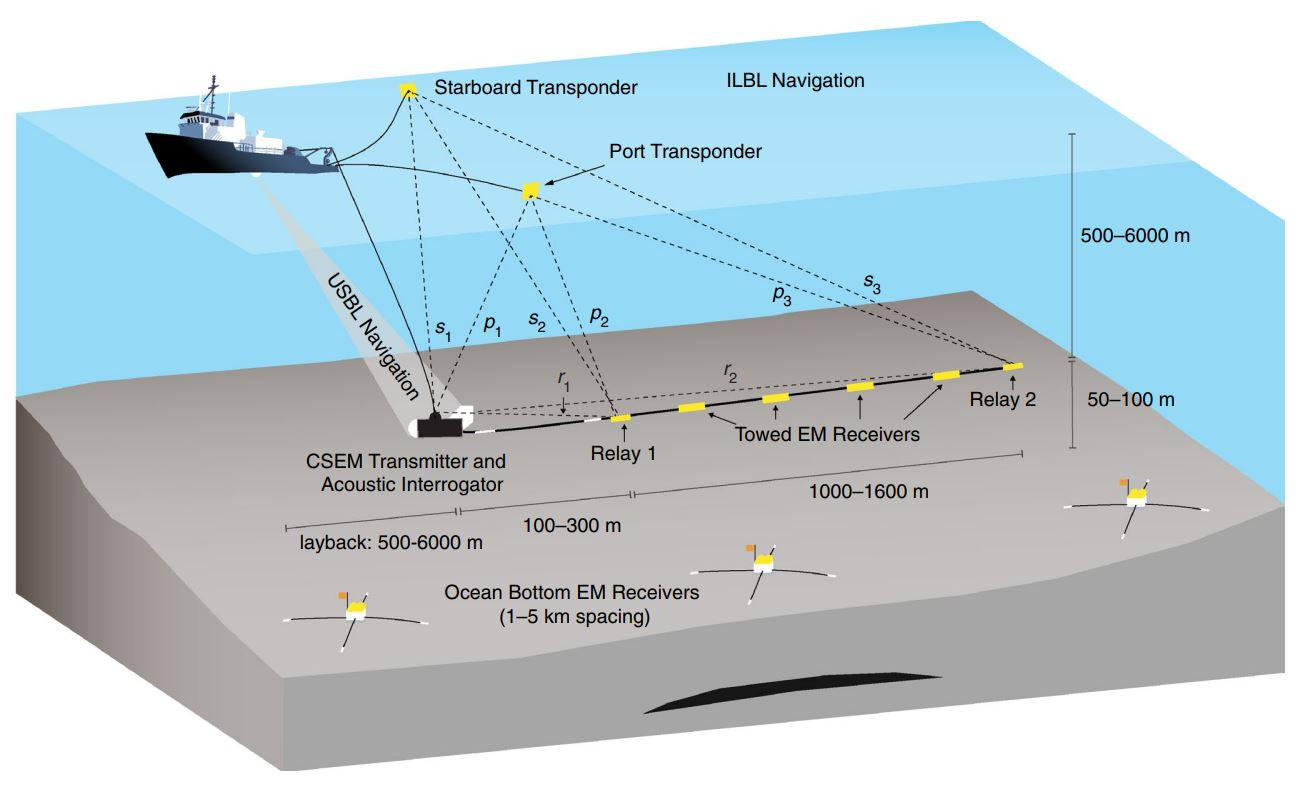
\includegraphics[width=0.75\textwidth]{ilbl}
	\caption{Inverted long baseline system example \cite{ilbl}}
	\label{fig:ilbl}
\end{figure}

In this thesis, an iSBL acoustic positioning system is proposed. While iUSBL systems primarily use phase-differencing (but not always) and a baseline of less than one wavelength, this proposed iSBL system will use time-differencing and a baseline of greater than one wavelength. The system also uses a single transmitter on the surface of the water (attached to a floating buoy or other autonomous vehicle) and an array of multiple receivers on the underwater vehicle. For a full underwater implementation of this iSBL system, it is recommended to place the receivers as far apart as possible on the body of the underwater vehicle as possible to increase the accuracy of the position estimate.

\subsection{Similar Implementations} \label{ssec:3s1s3}
While the classification of this system as an iSBL system is novel, the design of the system draws upon previous research. Since iUSBL and iSBL are quite similar, some iUSBL systems were studied and used as inspiration for this thesis. Luo and Ko of Hoseo University in South Korea designed an iUSBL system with a floating beacon on the surface of the water, and implemented more complex systems (such as simultaneous mapping and localization algorithms) into their design \cite{iusblukf}. Researchers from Zhejiang University in China implemented an iUSBL system on an autonomous underwater vehicle that uses FPGAs and beamforming to improve the position estimate \cite{passiveiusbl}.

The four most relevant implementations are as follows. Alcocer, Oliveira, and Pascoal from the Institute for Systems and Robotics of Portugal described an acoustic positioning system using GPS Intelligent Buoys (GIBs), which act like a floating LBL system with acoustic and GPS receivers on each buoy \cite{gibs}. Smith and Kronen of the Florida Atlantic University’s Department of Ocean Engineering detailed a low-cost SBL positioning system using a foldable acoustic array \cite{lowcostsbl}. More researchers from Zhejiang University in China created and tested a single-transmitter, variable-baseline acoustic positioning system, the most similar implementation to the one developed in this thesis \cite{singletrans}. Lastly, Morgado, Oliveira, and Silvestre from the Technical University of Lisbon, Portugal tested a USBL system with tightly-coupled inertial measurement devices, which combines the USBL position estimates with an inertial navigation system using an extended Kalman filter \cite{tightekf}.

Finally, a GitHub repository by the Underwater Communication and Navigation Laboratory provided many fantastic examples of acoustic positioning implementations. The UCNLNav repository was instrumental in this implementation, giving a great example of implementing Hooke-Jeeves search for time-difference-of-arrival systems \cite{ucnlnav}. This repository will be revisited later in Section \ref{ssec:3s9s2}.

\section{Receiver Array Mechanical Design} \label{sec:3s2}
The receiver array for this implementation is made of four ultrasonic transducers spaced in an X-pattern, with each transducer having a baseline of 25cm from the center. See Figure \ref{fig:isblnaked} for an image of the array without any wiring attached. The array is mounted at a 90° angle relative to the Fo-SHIP’s end effector, pointing towards the X-axis of the Fo-SHIP.

\begin{figure}[htbp]
	\centering
	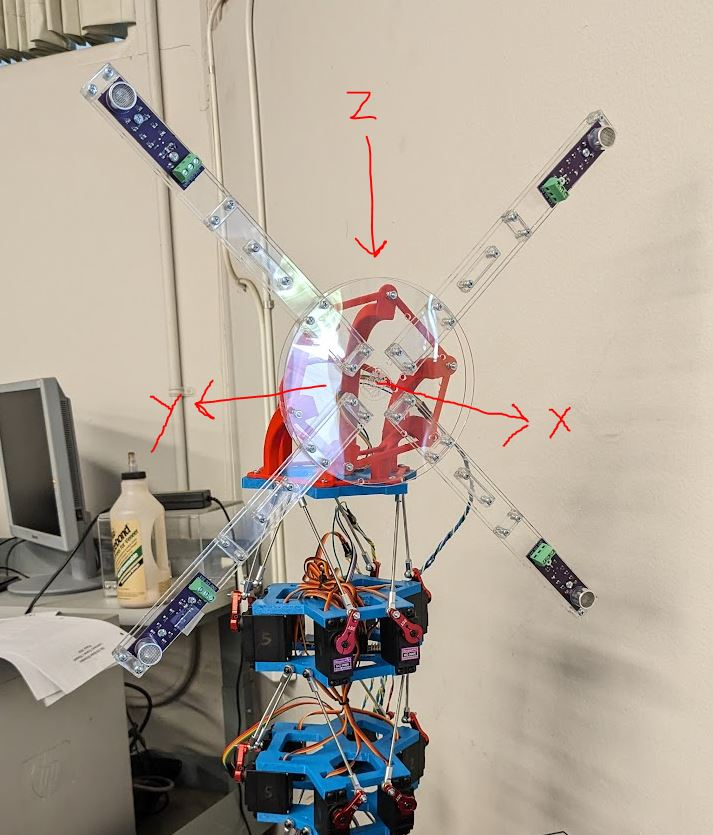
\includegraphics[width=0.5\textwidth]{isblnaked}
	\caption{iSBL array without wiring or microcontroller, with local coordinate system overlaid}
	\label{fig:isblnaked}
\end{figure}

The array is constructed from laser-cut 2.4mm-thick acrylic sheet. The components were designed using SOLIDWORKS and were cut on the Mustang ‘60 Machine Shop PLS laser cutters. Four long beams are attached to a central circular hub; the microcontroller, soldered breadboard, and IMU have mounting holes on the central hub, while the receivers have mounting holes on the ends of the long beams. The holes are spaced such that the center of the ultrasonic receiver elements are 25cm from the center of the array. A partial CAD model of the array can be seen in Figure \ref{fig:partarray}.

\begin{figure}[htbp]
	\centering
	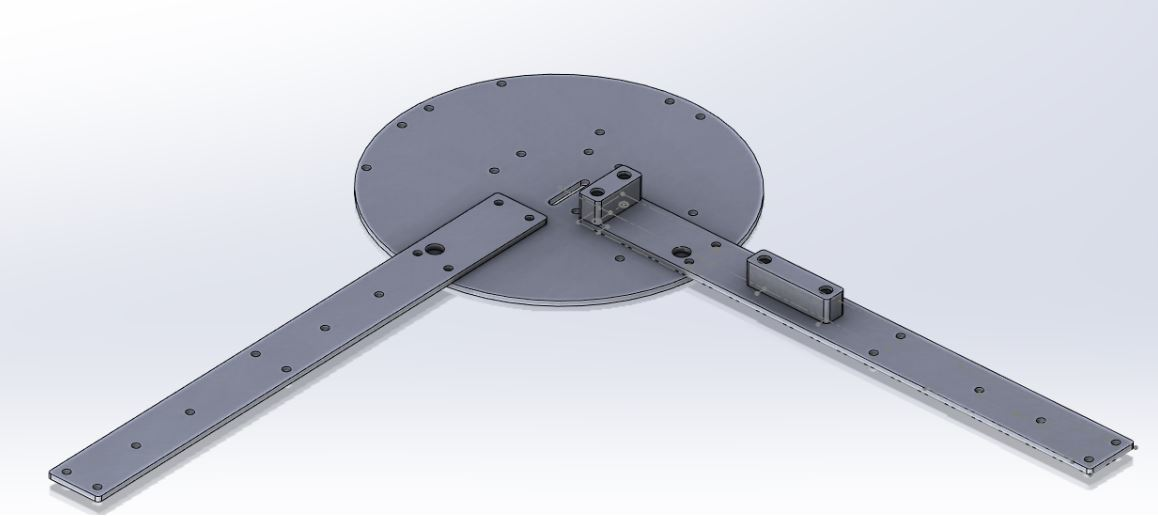
\includegraphics[width=0.8\textwidth]{partarray}
	\caption{Partial CAD model of iSBL array, made using SOLIDWORKS}
	\label{fig:partarray}
\end{figure}

Note that the array was constructed from multiple layers of planar acrylic components to reduce the weight of the iSBL array, which affects the overall loading on the Fo-SHIP end effector. The array uses spacer elements to allow for flexibility of the long members, which can help account for any warping of the long, thin elements. Additionally, acrylic sheeting was a low-cost, low-weight, and easy-to-manufacture component when compared to other materials like wood or aluminum. A side view of the array can be seen in Figure \ref{fig:sidearray}.

\begin{figure}[htbp]
	\centering
	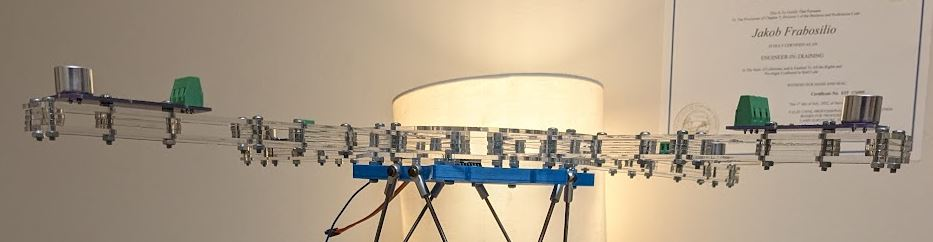
\includegraphics[width=\textwidth]{sidearray}
	\caption{Side view of iSBL array}
	\label{fig:sidearray}
\end{figure}

Lastly, a 90° adapter was printed on a Prusa Mk.3 FDM 3D printer in the Mustang ‘60 Machine Shop. This component is crucial for testing the iSBL-SF algorithm in a horizontal test environment. If the adapter was not added, then the Fo-SHIP would need to be mounted horizontally on a wall (poor loading condition due to gravity), or the transmitter element would need to be suspended in the air above the Fo-SHIP. The adapter was designed in Solidworks and incorporates many lightweighting and stiffening elements. A render of the adapter in 3D printing slicing software can be seen in Figure \ref{fig:sliceradapter}.

\begin{figure}[htbp]
	\centering
	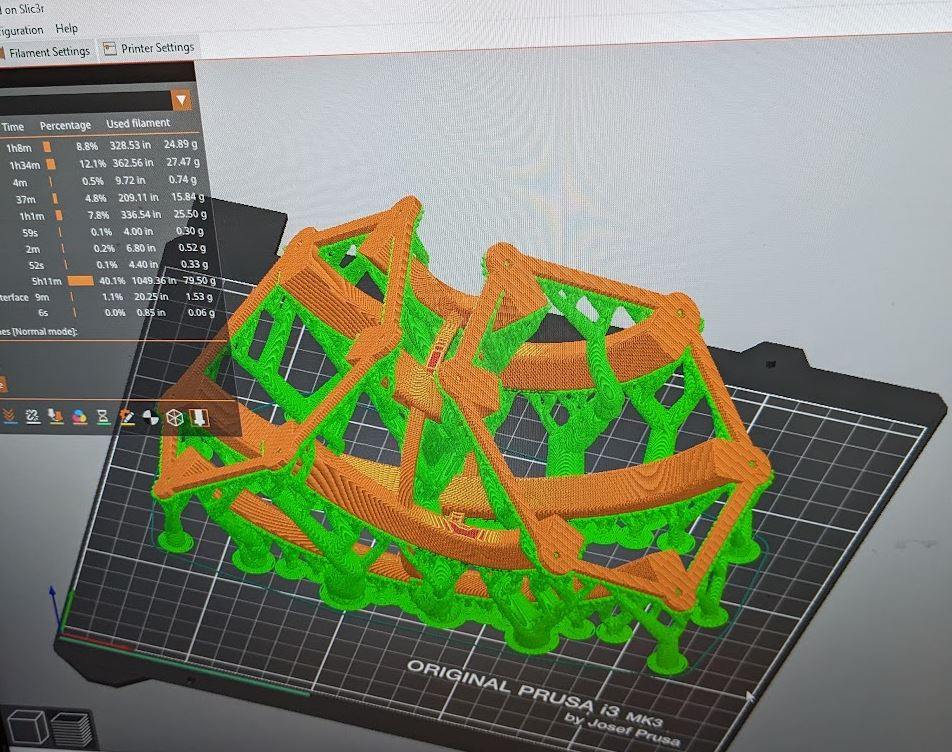
\includegraphics[width=0.6\textwidth]{sliceradapter}
	\caption{iSBL adapter in 3D slicing software (PrusaSlicer)}
	\label{fig:sliceradapter}
\end{figure}

\section{Receiver Array Electrical Design} \label{3s3}
The acoustic positioning system and iSBL array include three main components: the STM32 microcontroller, the receiver elements, and the IMU. The receiver element design is discussed in Section \ref{sec:3s4}, and the IMU selection is discussed in Chapter \ref{chap:4c}. For the rest of this chapter, it will be referred to as “the IMU,” but its full designation is a combined LSM6DSOX 3-axis accelerometer and gyroscope and LIS3MDL 3-axis magnetometer.

The microcontroller used for this project is the STM32H723ZG from STMicroelectronics. This microcontroller was chosen with specific requirements: an analog-to-digital converter (ADC) capable of recording more than 1 million samples per second at 12-bit resolution, random access memory storage greater than 200kB, digital signal processing libraries, and as high of a CPU clock speed as possible. The H723ZG fulfills all these requirements \cite{stmdatasheet}, comes on a development board for easy prototyping and implementation, and is very low-cost at around \$30 for one development board \cite{stm144}. The development board is much larger than required for this system with over 114 GPIO pins and 30 ADC channels, so for future implementations, switching to a custom printed circuit board (PCB) would be recommended. An image of the STM32H723ZG development board can be seen in Figure \ref{fig:stm144}.

\begin{figure}[htbp]
	\centering
	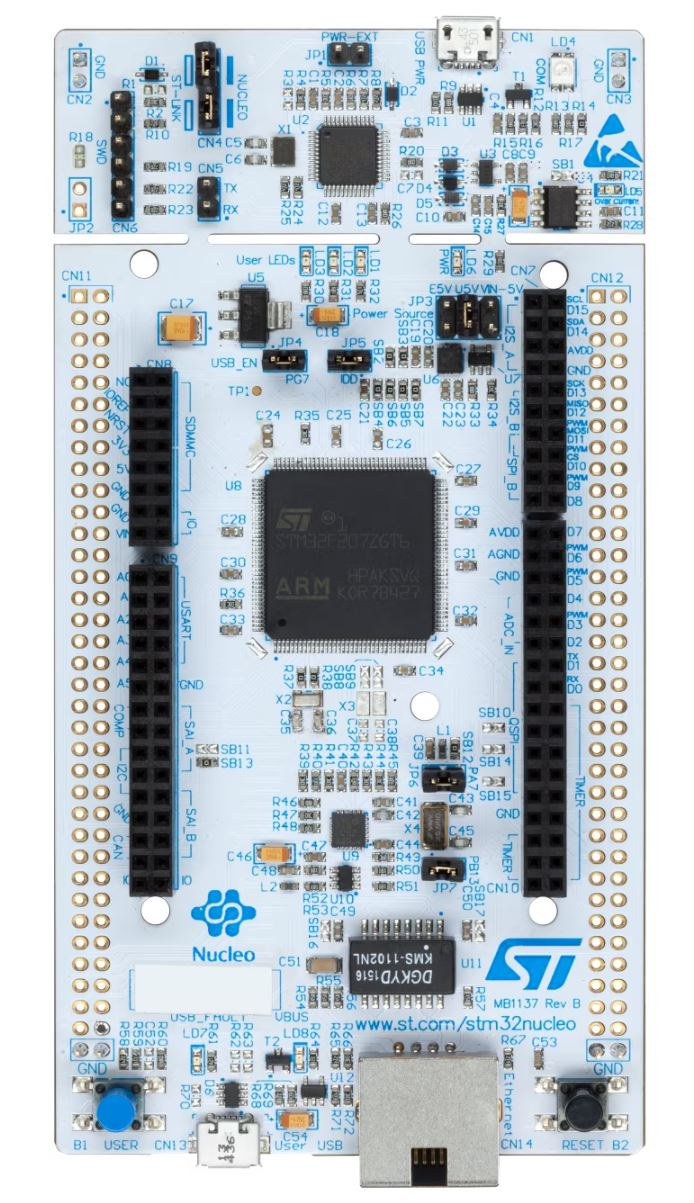
\includegraphics[width=0.35\textwidth]{stm144}
	\caption{STM32H723ZG development board \cite{stm144}}
	\label{fig:stm144}
\end{figure}

For this implementation, four ADC inputs, two GPIO pins, one USB connection, one I\textsuperscript{2}C connection, and one serial connection are used. A wiring diagram in Figure \ref{fig:stmwiring} shows the full schematic of the system. The STM32 communicates with the IMU over I\textsuperscript{2}C, communicates with a laptop via USB, and communicates with the ESP32 controlling the Fo-SHIP via a serial connection. The wiring and communications protocol for I\textsuperscript{2}C and serial are described in Section \ref{sec:2s3}. Each receiver element is connected to an ADC input, as well as a power and ground connection. Four LEDs are used for debugging and testing; three are internal LEDS on the STM32 development board, while one is connected to an external GPIO pin. A second GPIO pin is used as an interrupt for the IMU; when the IMU has new data ready, the STM32 can detect it via this GPIO pin.

\begin{figure}[htbp]
	\centering
	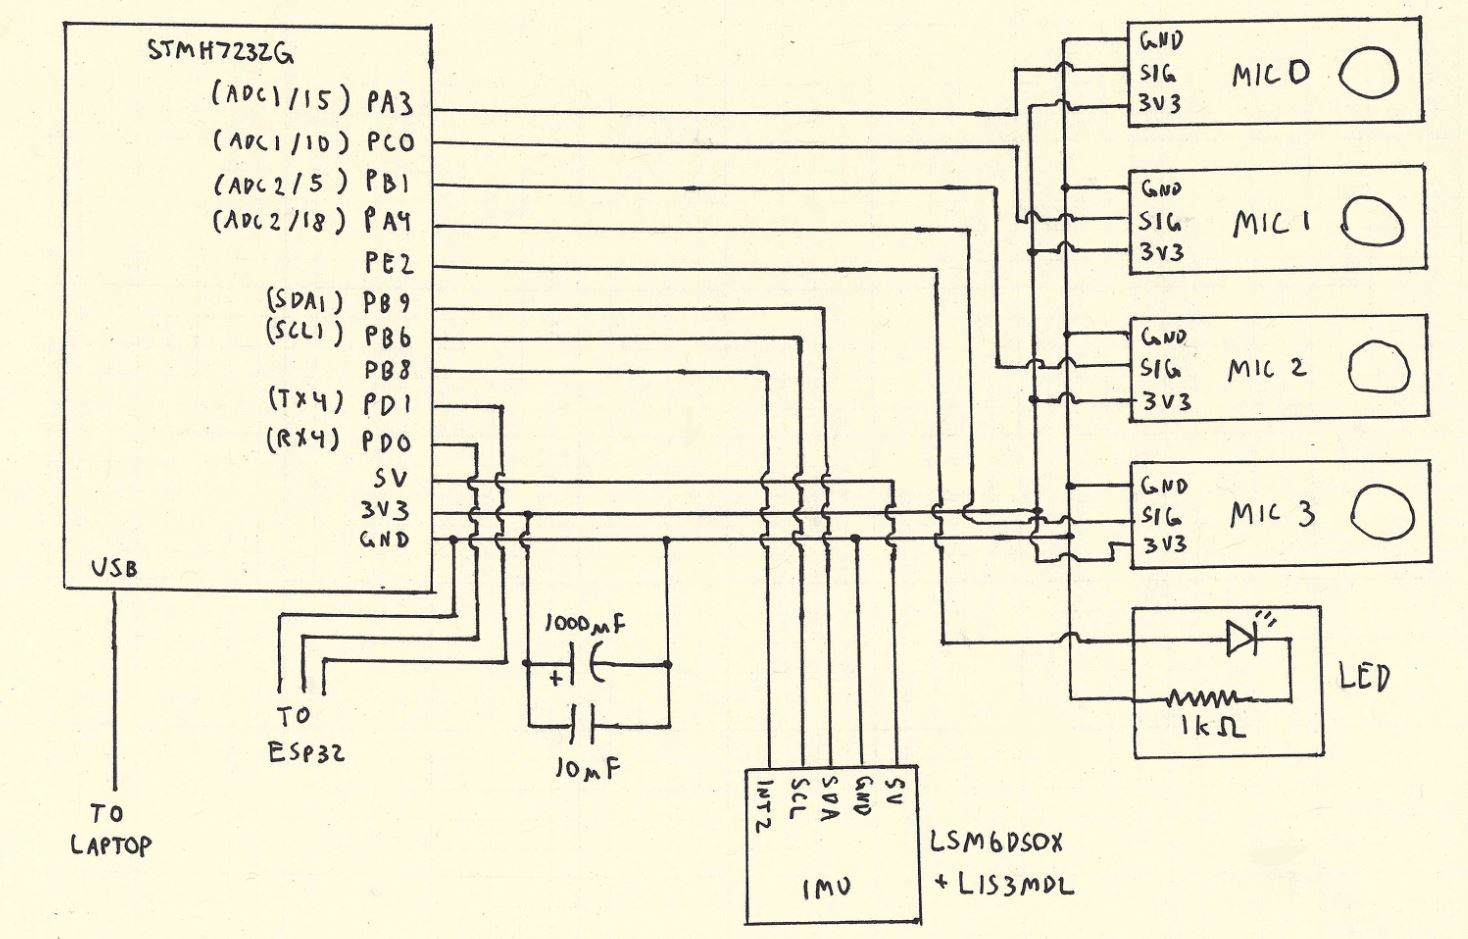
\includegraphics[width=\textwidth]{stmwiring}
	\caption{iSBL system wiring diagram}
	\label{fig:stmwiring}
\end{figure}

Lastly, two capacitors, one large 1000uF electrolytic capacitor and one small 10uF ceramic capacitor, were added to filter out electrical noise from the STM32’s 3v3 line. 

\section{Active Band-Pass Filter Design} \label{sec:3s4}
This implementation is designed to work with 40kHz audio signals. This frequency was chosen for a few reasons:
\begin{itemize}[noitemsep,topsep=0pt,]
	\item The above-water frequency should be similar to the planned underwater system’s frequency to allow for simple future implementation
	\item The audible range should be avoided to minimize disturbance to marine animals (see Section \ref{sec:6s4} for more details on the underwater system extrapolation)
	\item Lower frequencies require lower ADC sampling rates to record a single wave
	\item Lower audio frequencies attentuate much less rapidly in seawater compared to higher frequencies (see Figure \ref{fig:attenuation})
	\item 40kHz is a very common frequency for air-based ultrasonic transducers, and fairly common in water-based ultrasonic transducers
\end{itemize}

\pagebreak

\begin{figure}[htbp]
	\centering
	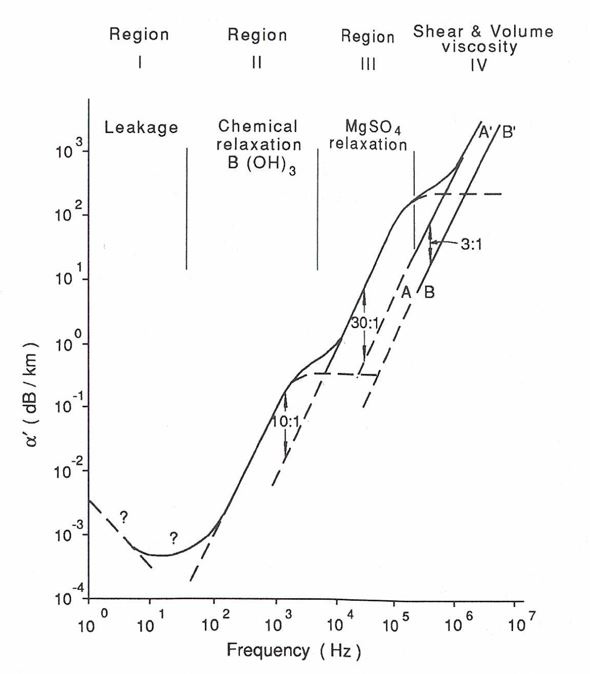
\includegraphics[width=0.65\textwidth]{attenuation}
	\caption{Sound attenuation in seawater with dominant attenuation process regions \cite{computational}}
	\label{fig:attenuation}
\end{figure}

Using ultrasonic transducers without any filtering or amplification would severely limit the range and accuracy of the acoustic positioning system. To overcome both of these issues, an electrical circuit is necessary to:
\begin{itemize}[noitemsep,topsep=0pt,]
	\item Amplify the output voltage of the receiver elements to a sufficient level for the microcontroller’s ADCs
	\item Reject frequencies that are outside of the desired passband
	\item Be inexpensive and scalable to all microphones
	\item Reduce the amount of digital pre-processing required
\end{itemize}

An active band-pass filter is a good solution to the problem and it fulfills the above requirements. Inverting active band-pass filters in particular are designed to have narrow pass-bands. An inverting active band-pass filter based on a circuit from ElectronicsTutorials \cite{abpfws} (see Figure \ref{fig:abpfws}) was used with the following modifications:
\begin{itemize}[noitemsep,topsep=0pt,]
	\item A decoupling capacitor and voltage divider (C3, R3, R4) that adds a 1.65V DC bias to the microphone signal
	\item A voltage divider (R5, R6) that sets the non-inverting input of the op-amp to 1.65V
\end{itemize}

\begin{figure}[htbp]
	\centering
	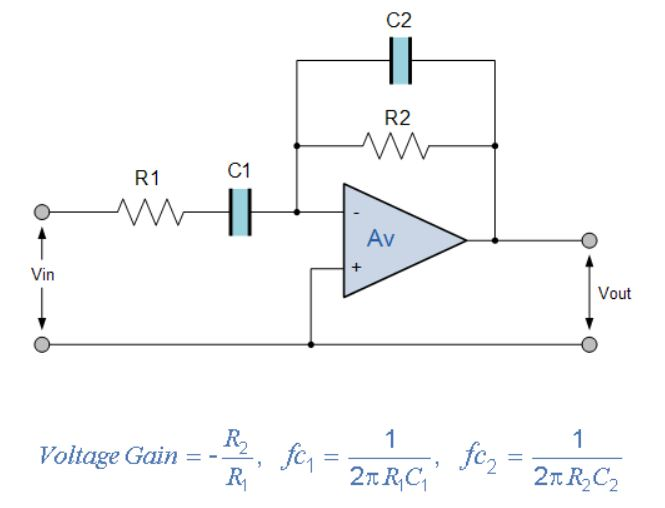
\includegraphics[width=0.8\textwidth]{abpfws}
	\caption{Inverting active band-pass filter \cite{abpfws}}
	\label{fig:abpfws}
\end{figure}

These modifications are necessary for the system to function - see the modified circuit diagram in Figure \ref{fig:abpfcircuit}. When testing an ultrasonic receiver and transmitter at a distance of 3 meters apart, the receiver registered a peak-to-peak voltage of approximately 10mV when the transmitter was powered by a 12Vpp, 40kHz sine wave. This voltage oscillates around 0V. The ADC on the STM32 is capable of reading voltages between 0V and 3.3V; to maximize the range of the receiver output, a 1.65V DC bias needs to be added to the receiver signal. Since the op-amp is being powered by an asymmetric 0V to 3.3V supply, the inputs must be biased to the center of the supply voltage range to minimize clipping at the rail voltages. This setup ensures that the whole range of the op-amp is used.

The resistor and capacitor values need to be carefully selected to provide proper filtering and amplification; the equations in Figure \ref{fig:abpfws} are the governing equations for this filter. First, a voltage gain of approximately 100 was desired to amplify the 10mVpp signal to 1Vpp; this resulted in a resistor ratio of 100:1. Next, cutoff frequencies as close to 38kHz and 42kHz were desired to reduce the amplification of frequencies outside of this passband. After many iterations of resistor and capacitor values (using common values from the E6 and E12 series to avoid using special components and to reduce cost \cite{e6e12}), the values in Figure \ref{fig:abpfcircuit} were chosen. These values result in a gain of -100 and cutoff frequencies of 38.1kHz and 41.3kHz. 

\begin{figure}[!htbp]
	\centering
	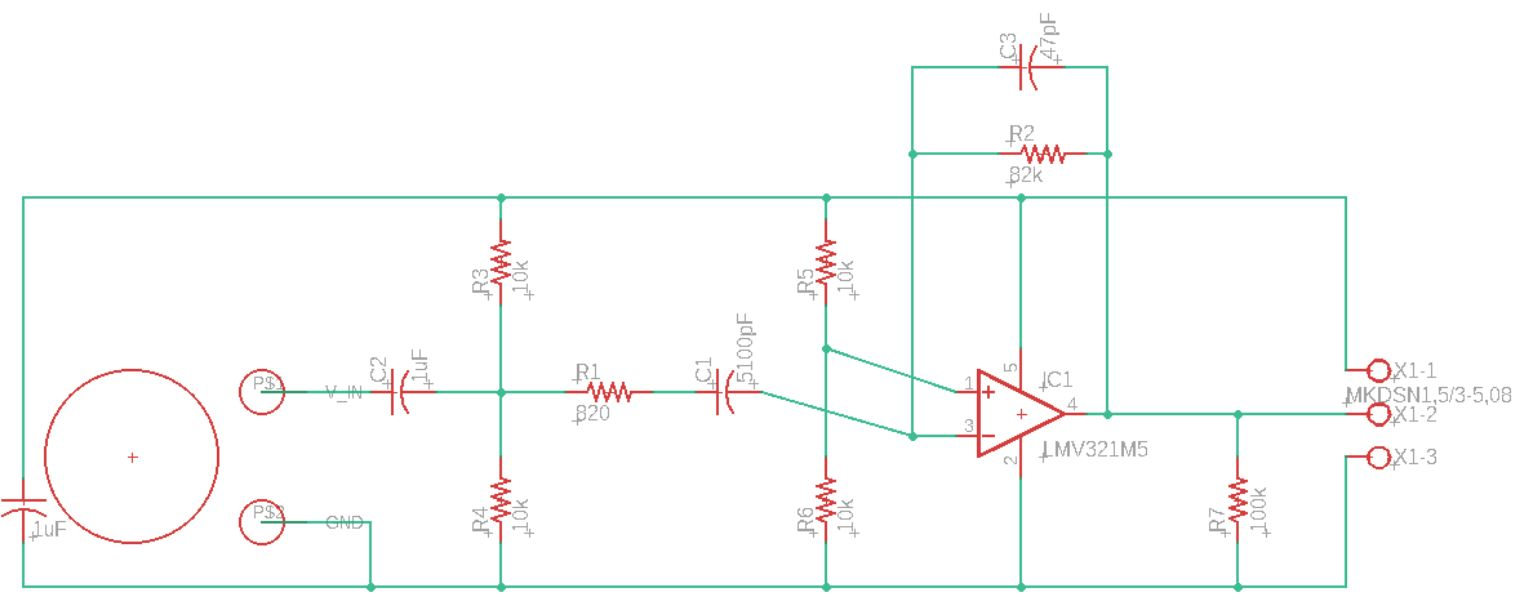
\includegraphics[width=\textwidth]{abpfcircuit}
	\caption{Custom active band-pass filter circuit diagram}
	\label{fig:abpfcircuit}
\end{figure}

The circuit was simulated in LTSpice, an electrical design and simulation software, to validate the design.. A sine sweep test with an AC source placed at the ultrasonic transducer element was run; the results can be seen in Figure \ref{fig:ltspice}. The simulation shows a peak amplitude response of 34.5dB at 39kHz, an approximate gain of 53. The filter does not have as sharp of a peak as desired, but the sensitivity curve of the ultrasonic receivers used has a similar curve; these two curves add together to produce a frequency response with a large peak at the resonant frequency of the receiver. See Figure \ref{fig:usrsens} for the sensitivity curve of the receiver.

\begin{figure}[htbp]
	\centering
	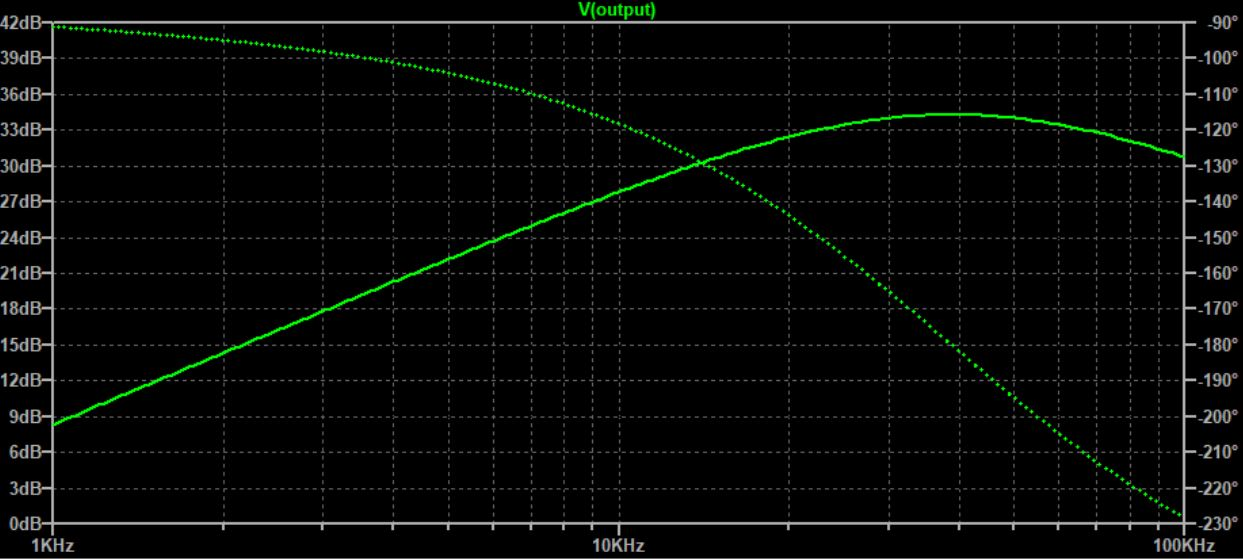
\includegraphics[width=\textwidth]{ltspice}
	\caption{Sine-sweep test of active band-pass filter circuit, run in LTSpice. Solid line is amplitude ratio, dashed line is phase shift}
	\label{fig:ltspice}
\end{figure}

\begin{figure}[htbp]
	\centering
	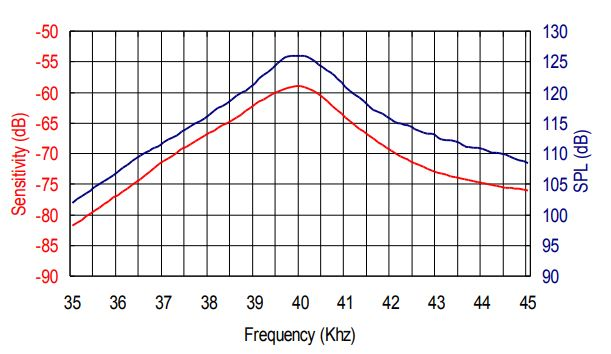
\includegraphics[width=0.6\textwidth]{usrsens}
	\caption{Sensitivity of 400SR160 ultrasonic receiver \cite{400sr160}}
	\label{fig:usrsens}
\end{figure}

\pagebreak

After selecting electrical components, the PCB files were designed in Eagle (see Figure \ref{fig:abpfeagleREAL}) and the PCB was then fabricated by OSH Park (a PCB manufacturer based in Oregon). See Figure \ref{fig:abpfeagle} for the rendering of the PCB from OSH Park. The electrical components for the circuit were purchased from Mouser Electronics.

\begin{figure}[htbp]
	\centering
	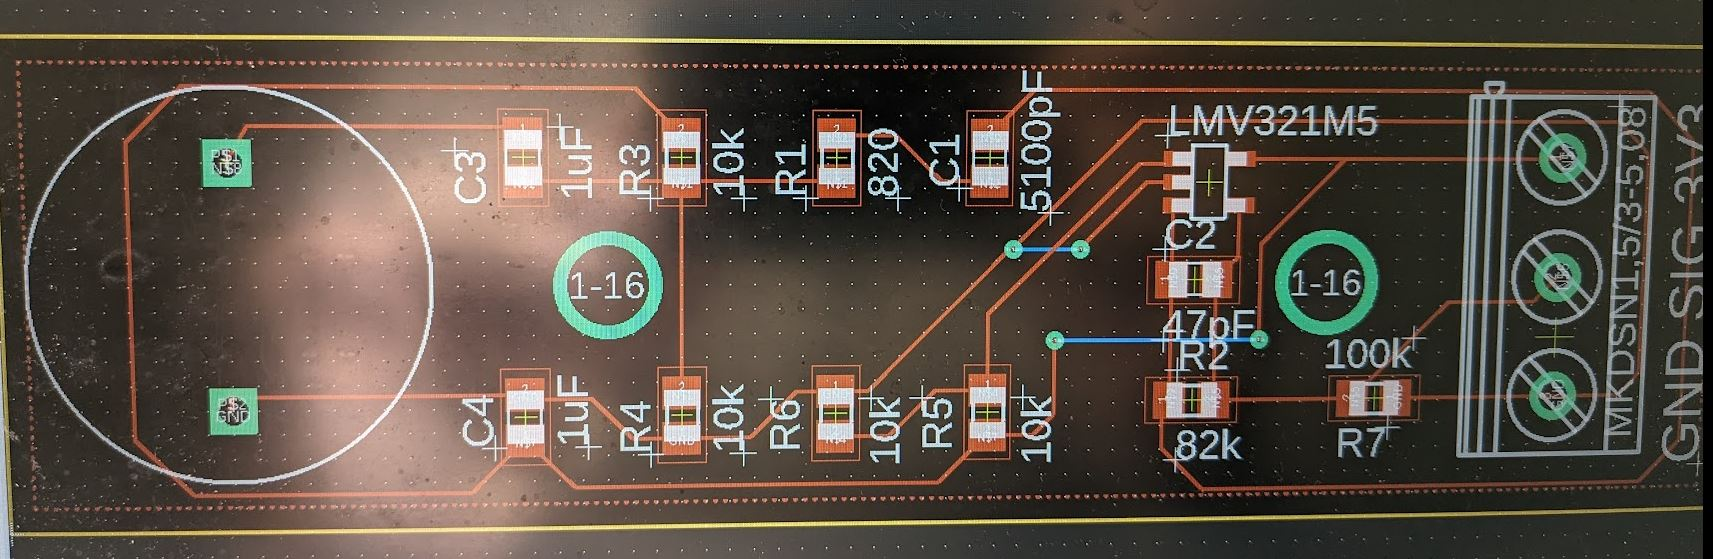
\includegraphics[width=0.7\textwidth]{abpfeagleREAL}
	\caption{Custom active band-pass filter in Eagle}
	\label{fig:abpfeagleREAL}
\end{figure}

\begin{figure}[htbp]
	\centering
	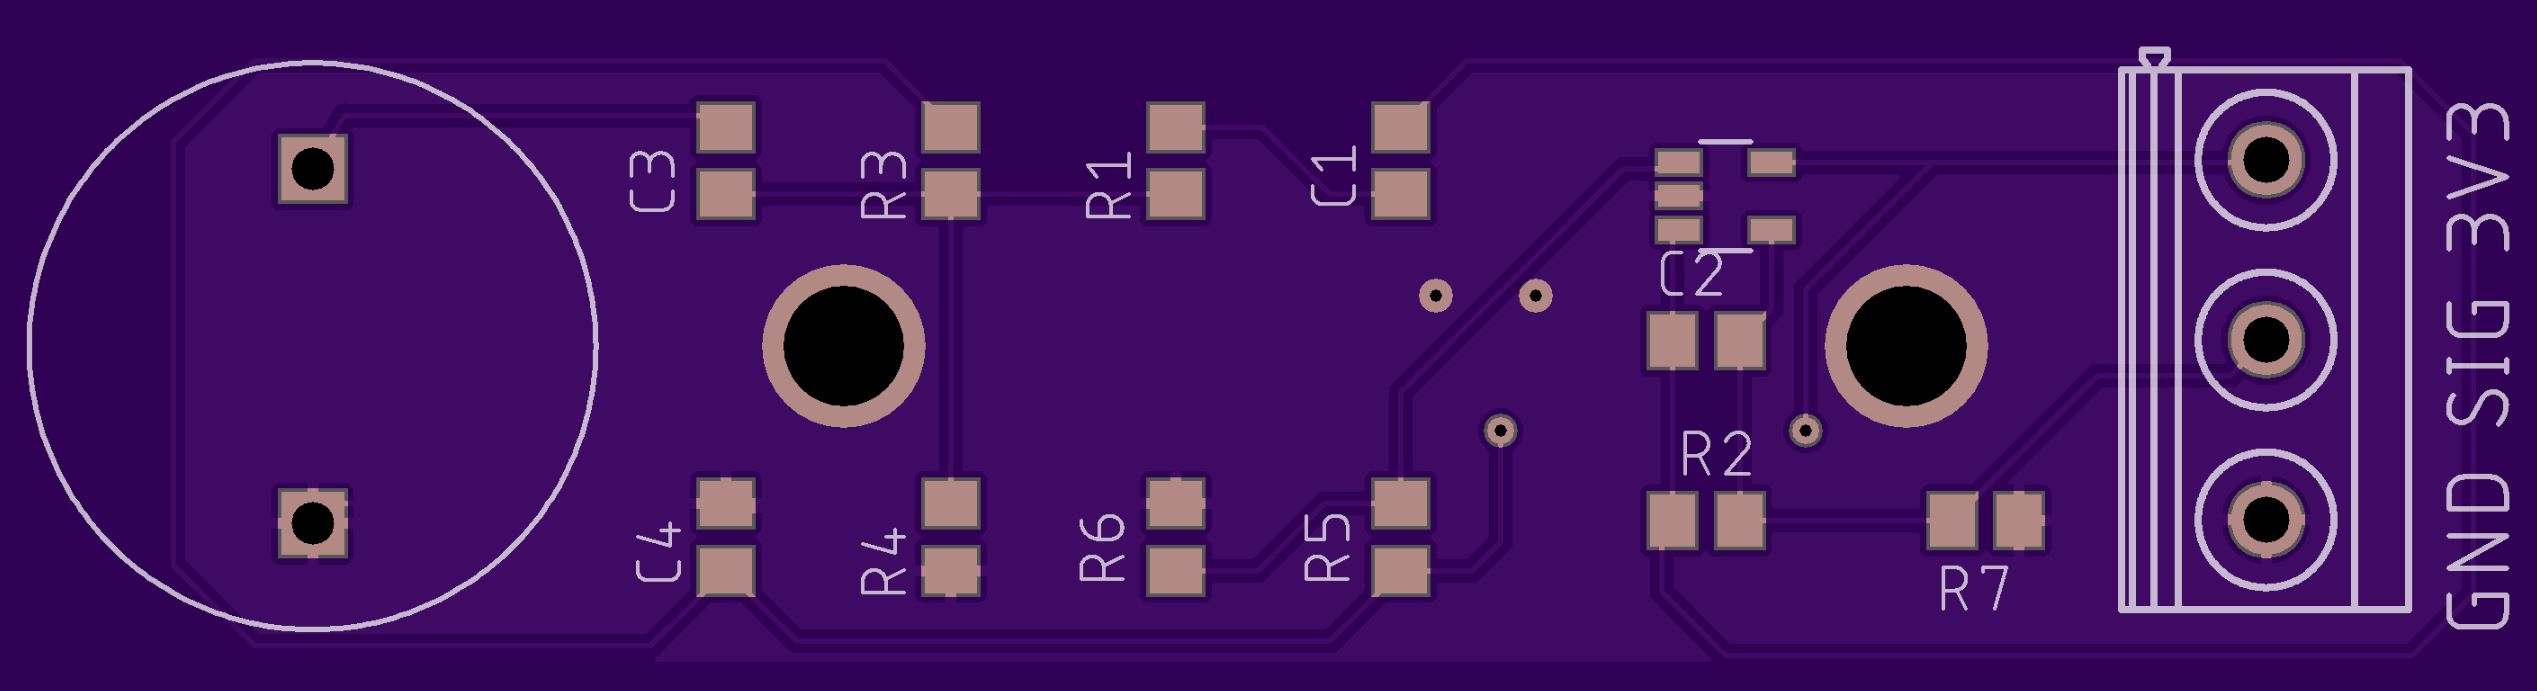
\includegraphics[width=0.7\textwidth]{abpfeagle}
	\caption{Custom active band-pass filter render from OSH Park order}
	\label{fig:abpfeagle}
\end{figure}

\begin{figure}[htbp]
	\centering
	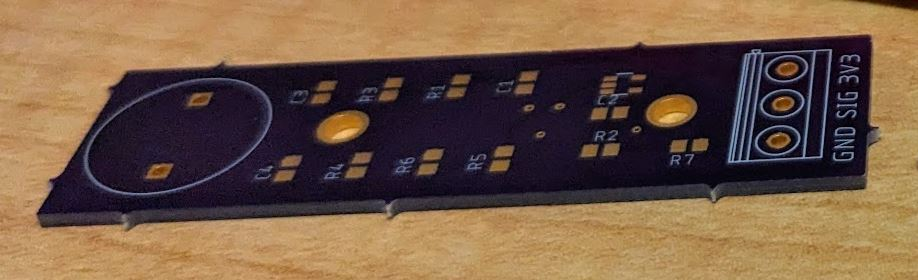
\includegraphics[width=0.7\textwidth]{abpfboard}
	\caption{Fabricated active band-pass filter PCB, unpopulated}
	\label{fig:abpfboard}
\end{figure}

\section{Receiver Array and PCB Assembly} \label{3s5}
The assembly process for the iSBL array involved soldering the PCBs and breadboard, assembling the acrylic frame, securing the electrical components to the acrylic frame, and attaching the array to the Fo-SHIP’s end effector.

First, the PCBs were assembled. After being delivered from Mouser, the electrical components were soldered to the PCBs; see Figure \ref{fig:abpfboard} for the PCBs before they were populated with components. All PCBs were hand-soldered using a soldering iron, heat gun, and solder wire. Figure \ref{fig:abpfmanu} shows one PCB in the process of being soldered, and Figure \ref{fig:abpffinished} shows a completed PCB. 

\begin{figure}[htbp]
	\centering
	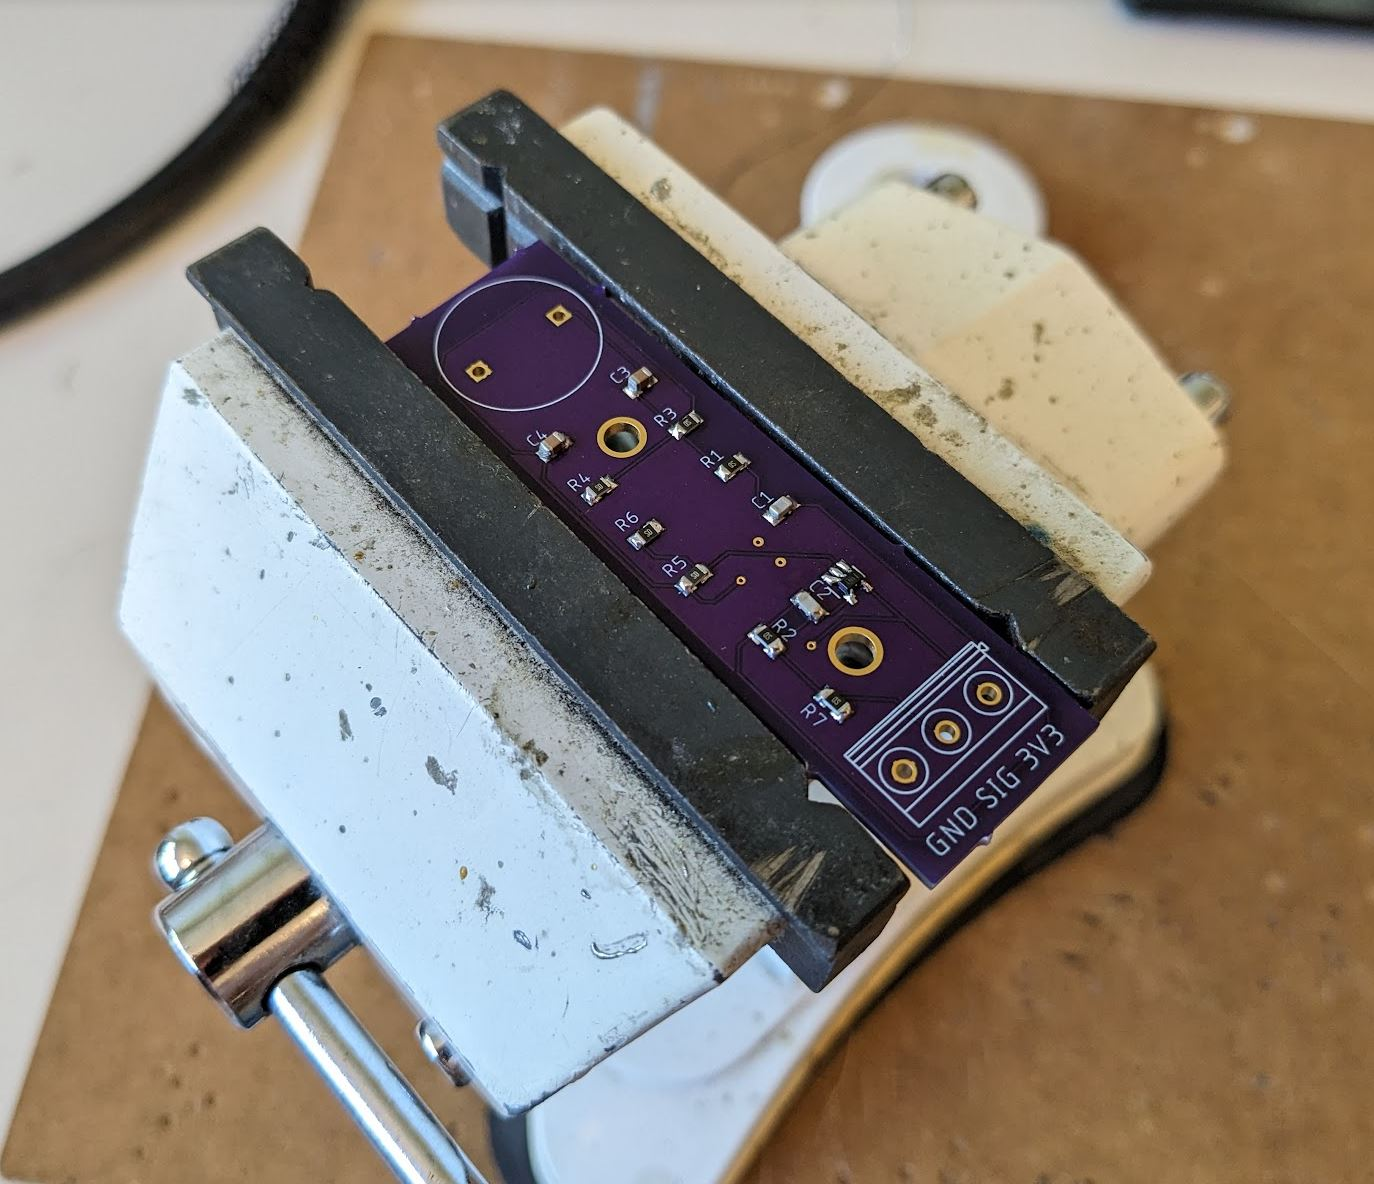
\includegraphics[width=0.58\textwidth]{abpfmanu}
	\caption{Soldering in-progess for PCB}
	\label{fig:abpfmanu}
\end{figure}

\begin{figure}[htbp]
	\centering
	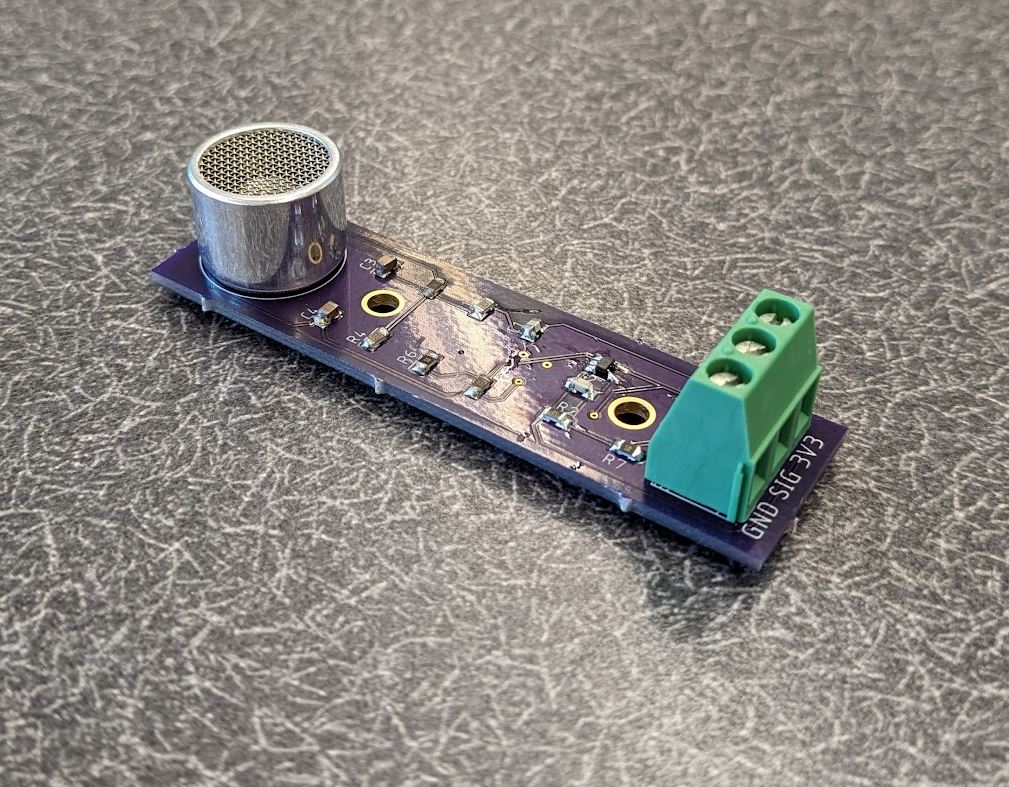
\includegraphics[width=0.58\textwidth]{abpffinished}
	\caption{Custom active band-pass filter render from OSH Park order}
	\label{fig:abpffinished}
\end{figure}

After this, the noise-reducing capacitors were soldered to a solderable breadboard. Header pins for each PCB signal line, as well as corresponding wires, were also soldered to the breadboard. Figure \ref{fig:breadboardstm} shows the breadboard. Note that three wires go from the breadboard to each PCB: ground, signal, and 3.3V power.

\begin{figure}[htbp]
	\centering
	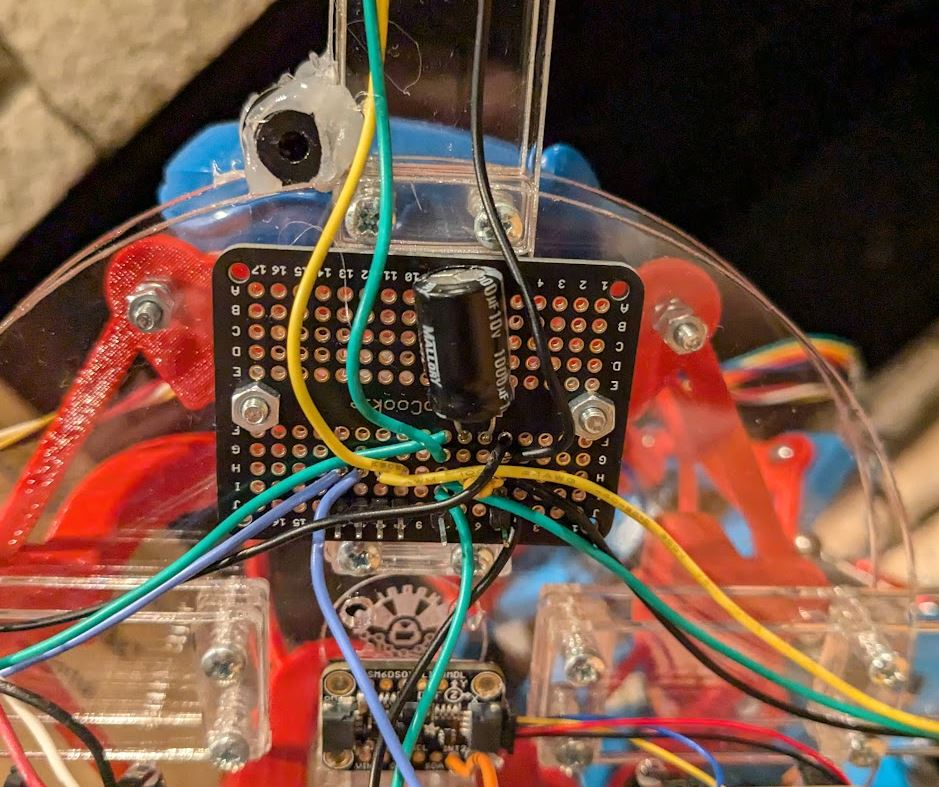
\includegraphics[width=0.55\textwidth]{breadboardstm}
	\caption{Soldered breadboard with capacitors, header pins, and wires to ultrasonic receiver PCBs}
	\label{fig:breadboardstm}
\end{figure}

\pagebreak

Next, the acrylic frame was assembled using the laser-cut acrylic components, M3x16 screws, and M3 nuts. Spacer plates were sandwiched between the long receiver arm plates and the central hub plates. The receiver PCBs and the soldered breadboard were secured to the acrylic using the M3 screws and nuts. Mounting holes for the IMU and the STM32 development board were not accessible during assembly due to poor planning - the STM32 is secured to the acrylic hub using cable ties, and the IMU is secured to the acrylic hub plate using adhesive. Two cable tie segments were cut from a single tie and placed on either side of the base of the IMU, and adhesive was placed in the space between the segments. This ensures that the IMU is parallel to the acrylic plate. All wiring was added between the STM32, breadboard, IMU, and receiver PCBs; loose wires were secured using cable ties. Lastly, the spacing between the ultrasonic receiver elements and the center was validated to be 25.0cm ± 0.1cm, and the spacing between individual receiver elements was validated to be 35.5cm ± 0.5cm

The final step of assembly was attaching the iSBL array to the Fo-SHIP end effector. The 3D-printed adapter was secured to the end effector using M3 screws; the iSBL array was secured to the adapter using additional M3 screws and nuts. All connections were tightened in a star pattern to avoid misalignments and to reduce the slop in the system. See Figure \ref{fig:isblfront} for the fully-assembled iSBL array.

\begin{figure}[htbp]
	\centering
	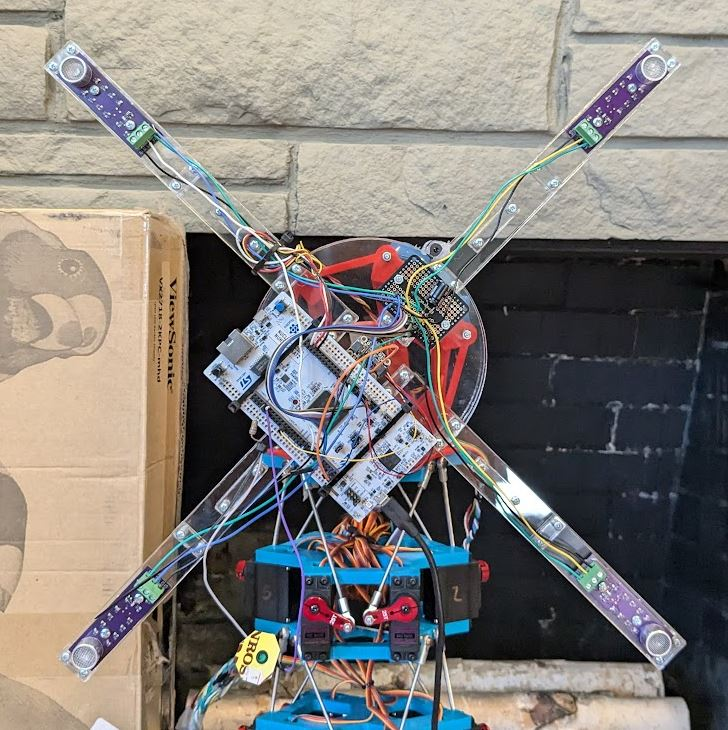
\includegraphics[width=0.85\textwidth]{isblfront}
	\caption{Fully-assembled iSBL array}
	\label{fig:isblfront}
\end{figure}

\section{Transmitter Design} \label{sec:3s6}
The purpose of the transmitter system is to send a particular acoustic pulse towards the receiver array using an ultrasonic transducer. This section details the hardware design of the transmitter, followed by the software design.

\subsection{Transmitter Hardware Design} \label{ssec:3s6s1}
The hardware design of the transmitter was one of the most iterated designs in this entire thesis. The basic design involves a microcontroller for generating a particular pulse, a motor driver (or other driver IC) to control the voltage across an ultrasonic transducer, and an ultrasonic transducer (single or multiple) to transmit the sound towards the receiver array. 

The microcontroller used is an STM32F411CEU6, on a development board commonly referred to as a “BlackPill” \cite{blackpill}. This microcontroller development board has a small form factor, is fairly low cost, and has high performance. Since the only physical connections to the microcontroller were two GPIO pins controlling the motor driver and a ground connection, the form factor was acceptable. Additionally, the microcontroller’s only function would be to generate a waveform (no multitasking), so extremely high performance like the STM32H723ZG provides would not be necessary.

The motor driver went through many iterations before finalizing a design. To work with the 40kHz transducers, it needed to have a switching frequency at or above 80kHz, and needed to provide up to 24Vpp at the voltage output. Initially, spare motor driver ICs were tested and deemed unfit for the purpose: a TPIC0107B motor driver had a switching frequency of 2kHz, far below the 80kHz required; an LM386 audio amplifier had a maximum output voltage of 12Vpp, which was half the maximum of the ultrasonic transducer’s range and did not produce a loud enough signal; an LM18298 motor driver had an adequate maximum output voltage, but only had a switching frequency of 25kHz; and an H-bridge constructed out of only P-type MOSFETs worked but wasted half its output power. Eventually, a spare motor driver made using optical switches by Charlie Refvem, one of the members of this thesis committee, was tested and performed fantastically. Many thanks to Charlie for loaning out the motor driver!

Lastly, the ultrasonic transducer chosen for this system is a 400ST160, manufactured by Pro-Wave Electronics Corporation \cite{400sr160}. This transducer has a center frequency of 40kHz and an acceptable beam angle of 55° at half-power. Two transducer configurations were tested: a single transducer, and a 3x3 array of transducers with 2.03cm spacing. The 3x3 array used a single input (all positive legs soldered together, and all negative legs soldered together); a phased array was considered, but was ultimately deemed out-of-scope. The array was simulated in Matlab (see Figure \ref{fig:matlab}) and shows a much shallower beam angle of approximately 7.5° for half-power. Experimentally, the 3x3 array delivered the same amount of acoustic energy at 28ft as a single transmitter did at 10ft; using the inverse square law for sound propagation, the 3x3 array has approximately 7.84x the power of a single transmitter, slightly less than the ideal 9x.

\begin{figure}[htbp]
	\centering
	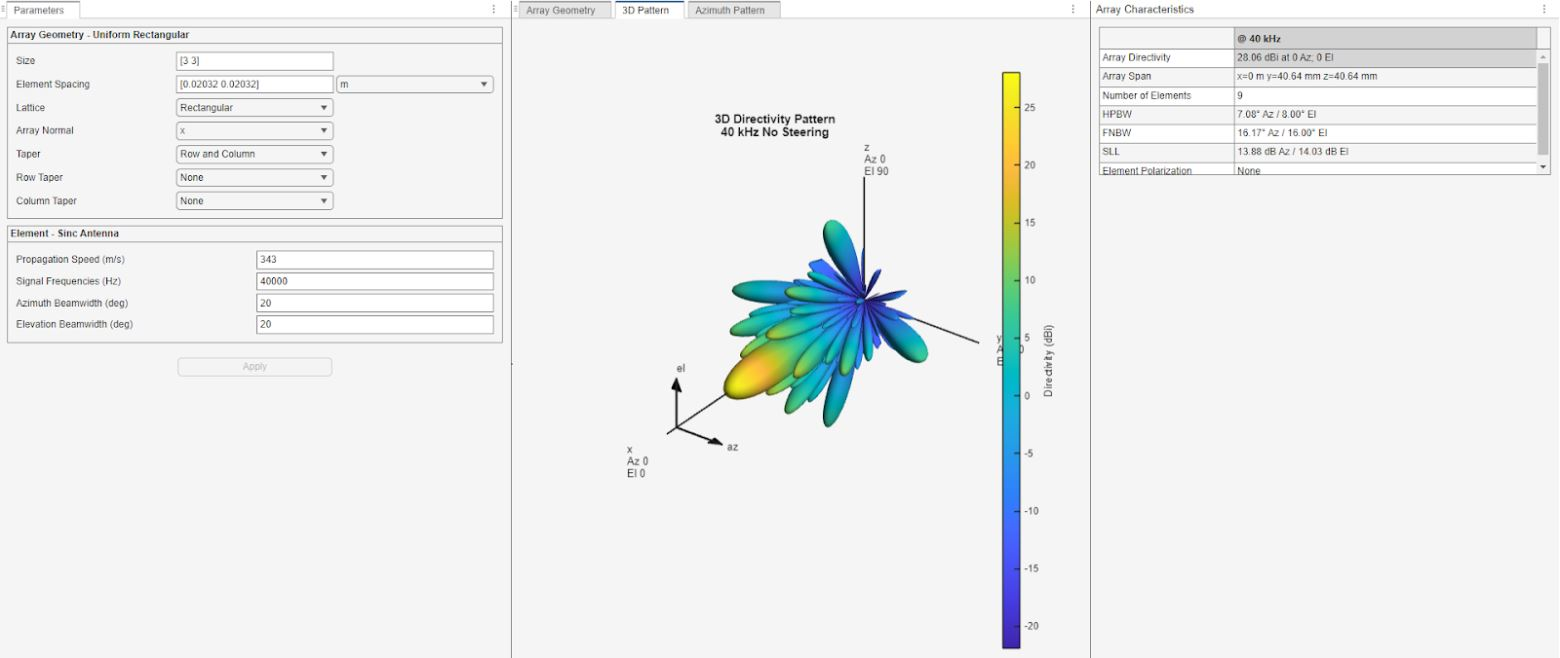
\includegraphics[width=1\textwidth]{matlab}
	\caption{MATLAB simulation of 3x3 array}
	\label{fig:matlab}
\end{figure}

Figure \ref{fig:txnine} shows an image of the fully assembled system, with the 3x3 array connected to the output of the motor driver. Ultimately, the much shallower beam angle of the 3x3 was producing poor results with the receiver array; the transmitter would need to be a minimum of 12.5ft away to hit each receiver element with a half-power pulse. Additionally, the array caused some phasing issues with the multiple transmitter elements, which ultimately produced a slightly different signal at each receiver. Since the acoustic model assumes a single transmitter and an identical (but time-shifted) signal at each receiver, the 3x3 array would not be ideal, and the single transmitter was used for the remainder of the testing for this thesis.

\begin{figure}[htbp]
	\centering
	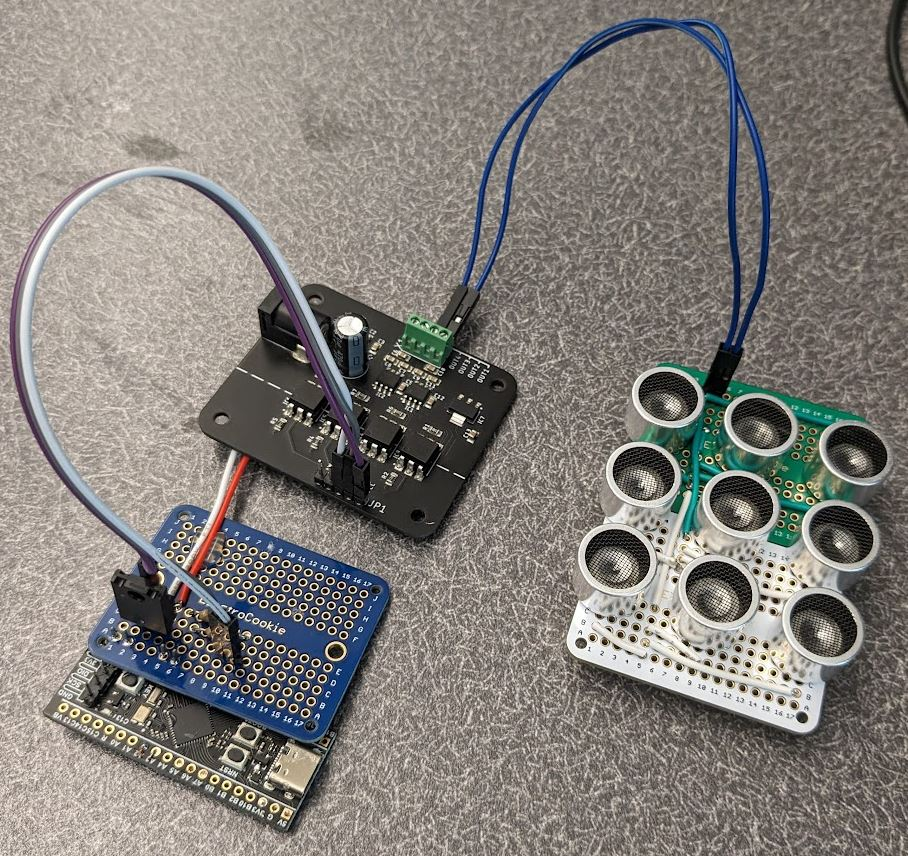
\includegraphics[width=0.65\textwidth]{txnine}
	\caption{Transmitter system with 3x3 array (eventually swapped with single transmitter)}
	\label{fig:txnine}
\end{figure}

\subsection{Transmitter Software Design} \label{ssec:3s6s2}
The STM32F411CEU6 was programmed using an ST-LINK/V2 from a spare Nucleo board. The code was developed in STM32CubeIDE, a software tool designed for programming STM32 microcontrollers. The code has two main functions: to generate a string of instructions for the motor driver, and to execute those instructions by toggling GPIO pins connected to the motor driver. 

Originally, a planned component of this thesis was to transmit GPS data over ultrasonic audio waves; an 8-bit character would be sent over ultrasonic, encoded using on-off keying, and then decoded using a neural network \cite{ultrann}. However, this was unable to be implemented into the thesis in time for submission. This functionality would allow the transmission of GPS coordinates from the transmitter buoy to the underwater vehicle, and is planned for future implementation.

First, the instructions are generated. This occurs once per second. An 8-bit character is chosen and converted to its binary representation and stored in a list. The first six bits of the list are a header; they are meant to trigger the receivers to start recording.

\begin{lstlisting}[language=C++]
message_int ++;			// pick the next number
message_int %= 256;		// between 0 and 255 (8-bit length),
message_char = (char)message_int;		// and save it as a char

// save in the last 8 bits of message_string
for(int i = 8; i > 0; i--){				
	message_string[14-i] = (message_int >> (i-1)) & 1;
}

message_string[0] = 1; 	// initialize the message with a header
message_string[1] = 1;
message_string[2] = 1;
message_string[3] = 1;
message_string[4] = 0;
message_string[5] = 0;
\end{lstlisting}

The \verb|message_string| is a list of 1s and 0s which will be transmitted using ultrasonic pulses - in a set time frame, one pulse denotes a 1 bit, and no pulse denotes a 0 bit. However, single pulses cannot be used for this case! Since the operating frequency is the same as the resonant frequency of the receivers, sending a single 40kHz wave would produce significant ringing in the transmitters. This ringing would affect data transmission rates if attempting to transmit bits over audio; additionally, sharper impulses provide the best results for time-differencing (as performed in Section \ref{sec:3s8}), so reducing the ringing is a primary concern.

A paper by researchers in the United Kingdom details a method for reducing this ringing by implementing active damping \cite{activedamping}. Figure \ref{fig:activedamping} shows two active damping waveforms and their results compared to a single transmitter pulse. Note that the second waveform produces an 80.7\% decrease in the length of the received pulse.

\begin{figure}[htbp]
	\centering
	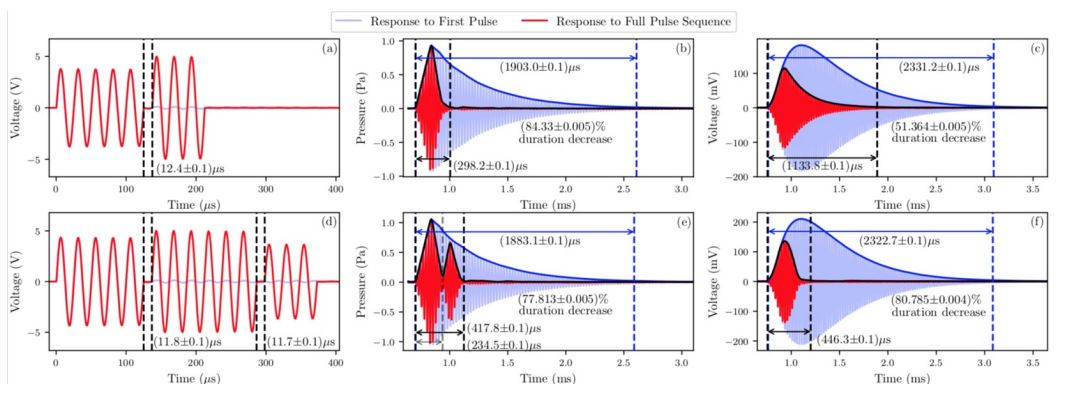
\includegraphics[width=1\textwidth]{activedamping}
	\caption{Active damping of ultrasonic receivers using engineered waves \cite{activedamping}}
	\label{fig:activedamping}
\end{figure}

\pagebreak

In the paper, the researchers are working with 40.01kHz audio waves. The second waveform shows a delay of 11.75us between sets of waves; these are approximately (but not perfectly) delays of half a wavelength. To simplify implementation, this thesis uses a modified waveform from the researchers’ second waveform: five 40kHz waves, one half-phase delay, six 40kHz waves, one half-phase delay, and three 40kHz waves. 

This modified waveform was implemented in the microcontroller code. The optical sensor motor driver takes in two inputs, A and B. A truth table for the motor driver can be seen in Table \ref{tab:truth} below. The positive lead of the transducer is connected to Out1 and the negative lead is connected to Out2. By holding the same voltage across both leads, the motion of the transducer is halted; by oscillating between the second and third row of the truth table at 80kHz, a 40kHz square-wave can be generated to drive the transducer.

\begin{table}[htbp]
	\centering
	\caption{Truth table for motor driver}
	\label{tab:truth}
	\begin{tabular}{|c|c|c|c|}
		\hline
		Logic level, InA & Logic level, InB & Voltage, Out1 & Voltage, Out2 \\
		\hline
		0 & 0 & 0V & 0V \\
		\hline
		0 & 1 & +12V & 0V \\
		\hline
		1 & 0 & 0V & +12V \\
		\hline
		1 & 1 & +12V & +12V \\
		\hline
	\end{tabular}
\end{table}

In the code, two lists are defined: \verb|on_a_string| provides a list of logic levels for InA, and \verb|on_b_string| provides a list of logic levels for InB. If the GPIO pins connected to these inputs are set to the instructions in these lists at a rate of 80kHz, a square version of the modified waveform is produced. See Figure \ref{fig:modwave} for the waveform produced by the GPIO pins when the code is run. A sinusoidal waveform was attempted and would produce better results, but the square waveform requires a much slower update rate and produced acceptable results at the receiver. Note that trailing ones are set to allow an appropriate delay between subsequent pulses.

\pagebreak

\begin{lstlisting}[language=C++]
/**< list of GPIO ODR instructions to send a 1 bit over audio, positive input to motor driver */
uint8_t on_a_string[] = {
	1, 0,
	1, 0,
	1, 0,
	1, 0,
	1, 0,
	1,	
	1, 0,
	1, 0,
	1, 0,
	1, 0,
	1, 0,
	1, 0,
	1,
	1, 0,
	1, 0,
	1, 0,
	1, 1, 1, 1, 1, 1, 1, 1, 1, 1};

/**< list of GPIO ODR instructions to send a 1 bit over audio, negative input to motor driver */
uint8_t on_b_string[] = {
	0, 1,
	0, 1,
	0, 1,
	0, 1,
	0, 1,
	1,
	0, 1,
	0, 1,
	0, 1,
	0, 1,
	0, 1,
	0, 1,
	1,
	0, 1,
	0, 1,
	0, 1,
	1, 1, 1, 1, 1, 1, 1, 1, 1, 1};
\end{lstlisting}

\begin{figure}[htbp]
	\centering
	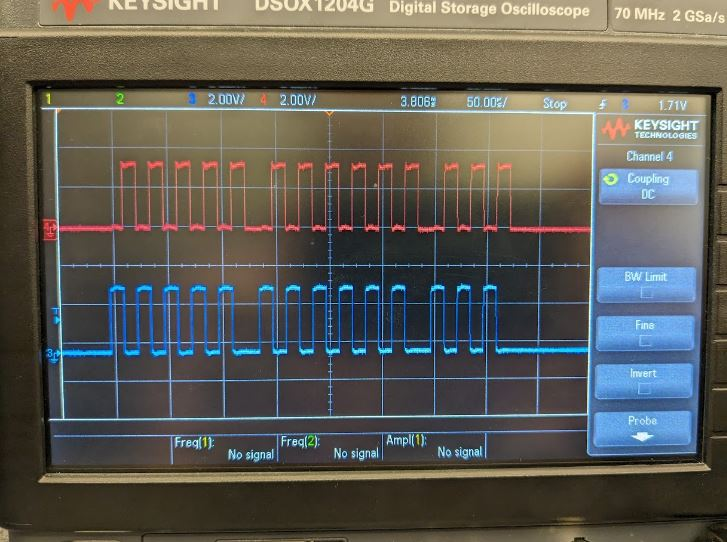
\includegraphics[width=0.75\textwidth]{modwave}
	\caption{Output of GPIO pins producing square waveform, input to motor driver}
	\label{fig:modwave}
\end{figure}

Now, the \verb|message_string| generated previously is combined with the above strings to produce a list of instructions. This list of instructions, \verb|driver_string|, details what the GPIO port associated with the motor driver pins should set its output data register (ODR) to every 11.25us. For every 1 bit in \verb|message_string|, it fills the \verb|driver_string| with the instructions in \verb|on_a_string| and \verb|on_b_string|. For every 0 bit in \verb|message_string|, it fills the \verb|driver_string| with an equivalent number of zeros. The code assumes that InA is connected to pin B6 and InB is connected to pin B7 on the STM32F411CEU6.

\pagebreak

\begin{lstlisting}[language=C++]
int index = 0;
for (int i = 0; i < sizeof(message_string); i++) {
	if (message_string[i] == 1) {
		for (int j = 0; j < sizeof(on_a_string); j++) {
			driver_string[index] = (on_a_string[j] << 6) | (on_b_string[j] << 7);
			index++;
		}
	} else {
		for (int j = 0; j < sizeof(on_a_string); j++) {
			driver_string[index] = 0;
			index++;
		}
	}
}
\end{lstlisting}

After the message is generated, a timer is started that updates at 80kHz. Every update, the GPIO ODR is set to the next value of \verb|driver_string|. Since each message bit takes 40 cycles of an 80kHz timer to send, the effective data rate of the transmission is approximately 2kHz. This means that in an ideal environment, data can be sent from the transmitter to the receiver at 2kb/s. Figure \ref{fig:oscope11110001} shows the 8-bit number 241, represented in binary as 11110001, as received by the iSBL receiver array.

\begin{lstlisting}[language=C++]
if (htim->Instance == TIM4){
	GPIOB->ODR = driver_string[instruction_counter]; 
	instruction_counter++;
	if (instruction_counter >= DRIVER_STRING_LEN){
		instruction_counter = 0;
		HAL_TIM_Base_Stop(&htim4);
	}
}
\end{lstlisting}

\begin{figure}[htbp]
	\centering
	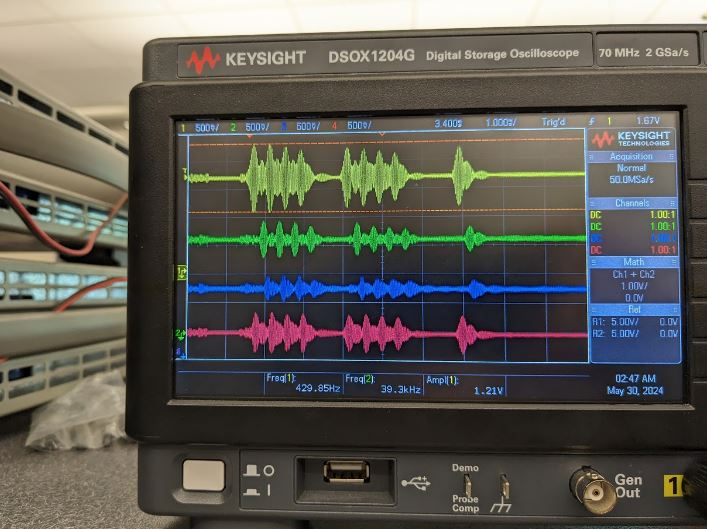
\includegraphics[width=0.75\textwidth]{oscope11110001}
	\caption{8-bit number 241 (11110001) transmitted over ultrasonic}
	\label{fig:oscope11110001}
\end{figure}

This process repeats once per second. Though the transmitter sends a message with multiple individual 40kHz pulses and 14 data bits, the transmission sent every second will be referred to as “a single acoustic pulse” for the remainder of this paper.

\section{Recording an Audio Pulse} \label{sec:3s7}
This section is the first of three detailing the acoustic position estimate code running on the STM32H723ZG. This first section details the overall finite-state machine diagram for the system, how the ADC is configured for MultiMode, the two different recording states (triggering and full recording), and how a “good” pulse is determined.

\subsection{Finite-State Machine} \label{ssec:3s7s1}
Figure \ref{fig:isblfsm} shows the finite-state machine representation of this system. There are five main states: initialization, triggering, full recording, recording validation, and data processing.

\begin{figure}[htbp]
	\centering
	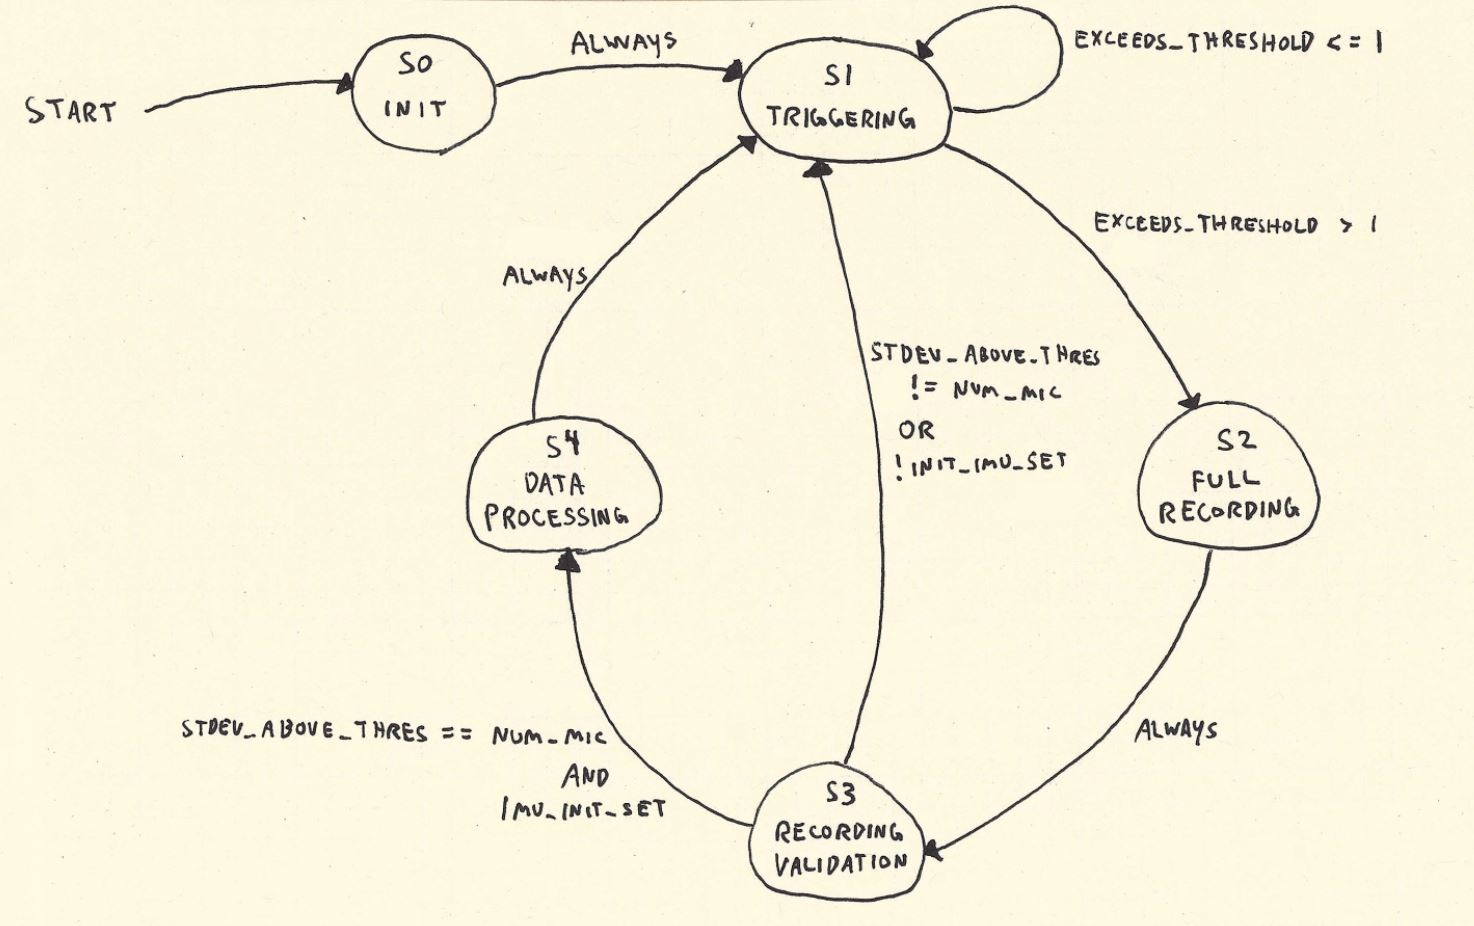
\includegraphics[width=\textwidth]{isblfsm}
	\caption{Finite-state machine diagram for acoustic positioning system}
	\label{fig:isblfsm}
\end{figure}

In the initialization state, three timers are started: TIM13 is used to count the time between Madgwick filter updates (see Section \ref{sec:4s4}), TIM14 is used to count the time between acoustic position updates (see Section \ref{sec:5s2}), and TIM3 is used to trigger ADC conversions (see Section \ref{ssec:3s7s2}). In this state, the first ADC conversion is started and the system moves into the triggering state.

In the triggering state, a small number of samples are recorded from each microphone (64, in this implementation). These samples are tested to see if they exceed a threshold defined by \verb|TRIG_THRES|. If more than one microphone exceeds the threshold, then the system moves to the full recording state. Otherwise, the system re-enters the triggering state. This state is crucial for detecting the header bits of an acoustic pulse and triggering the full recording process; without this step, a total of 2048 samples per microphone would need to be checked constantly. See Section \ref{ssec:3s7s3} for details on the triggering state.

In the full recording state, 2048 samples are recorded from each microphone (roughly 2.4ms of recording time, which is a good portion of a full 7ms acoustic pulse). The system does not update the IMU during this state to prevent any signal interference or cross-talk. After the recording buffer is full, the system transitions to the recording validation state.

In the recording validation state, the mean and standard deviation of each microphone’s signal is calculated. If all the standard deviations exceed \verb|TRIG_THRES| and the IMU has initialized, then the system moves to the data processing state. If either of these conditions are not met, the system restarts at the triggering state. See Section \ref{ssec:3s7s4} for details on the full recording and recording validation states.

In the data processing state, a position estimate is formed. First, the time shift between the microphone signals is calculated using FFT cross-correlation (see Section \ref{sec:3s8}). Next, the position of each microphone in the acoustic array is rotated by the current orientation of the platform (see Section \ref{ssec:3s9s1}) Then, the position of the transmitter relative to the receiver array is estimated using Hooke-Jeeves search using an acoustic propagation model (see Section \ref{ssec:3s9s2}). This relative position estimate is combined with the known position of the transmitter to give a position estimate of the receiver array (see Section \ref{ssec:3s9s3}). Finally, the acoustic position estimate and the dead reckoning position estimate are combined using Kalman filters (see Chapter \ref{chap:5c}).

In the background, linear acceleration, angular velocity, and magnetic field strength data are being recorded from the IMU at 208Hz. This data is then converted into an orientation estimate using a Madgwick filter, and into a position estimate using dead reckoning. See Chapter \ref{chap:4c} for details.

\subsection{ADC Configuration} \label{ssec:3s7s2}
The sampling rate of the ADC determines the resolution of the time shift calculation. The time shift between two signals sampled at 80kHz can only be determined to within 12.5us; assuming audio signals in water with a speed of sound of 1500 m/s \cite{computational}, this means that the distance from each microphone to the transmitter can only be discerned to within 9.4mm. This shift is enough to introduce significant error into the position estimation algorithm, so increasing the sampling rate of the ADC is a primary concern.

The ADC has multiple resolutions to choose from (8-bit, 12-bit, 16-bit, etc.). After testing, 12-bit resolution was found to provide enough resolution for the filtered audio signals with a resolution of approximately 0.81mV per bit. A single 12-bit ADC conversion takes approximately 12.5 cycles to convert on the STM32 \cite{stmdatasheet}, and higher resolutions take even longer.

Due to the input impedance of the active band-pass filter PCBs, additional ADC cycles were needed to stabilize the voltage output of the filter PCBs. Different sampling times were tested, and 8.5 cycles per conversion was found to provide a stable signal without requiring excess sampling time. Running at the maximum ADC clock speed of 50MHz and combining the standard conversion time of 12.5 cycles with the additional sampling time of 8.5 cycles, it takes approximately 0.42us to complete a single ADC conversion for one microphone.

Initially, only one ADC on the microcontroller was used for all four microphones. When the timer TIM3 updated, it would trigger a series of four subsequent conversions, one from each microphone. See Figure \ref{fig:adctimingsingle} for a timing diagram of these conversions. Since all four conversions happened subsequently, the maximum theoretical sampling rate for the ADC was approximately 595kHz. In practice, 500kHz was the maximum possible sampling rate - anything above this rate produced incomplete conversions for the final channel.

\begin{figure}[htbp]
\centering
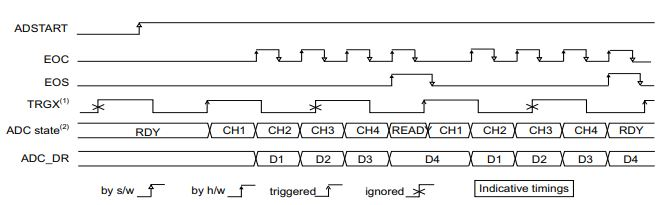
\includegraphics[width=\textwidth]{adctimingsingle}
\caption{Timing diagram for four subsequent ADC conversions \cite{stmdatasheet}}
\label{fig:adctimingsingle}
\end{figure}

However, using a configuration called MultiMode (also called "dual ADC" mode) allows the sampling rate to be doubled. In this configuration, one ADC (ADC1) is designated as the primary ADC, and a different ADC (ADC2) is designated as the secondary ADC. When the primary ADC is triggered, it then automatically triggers the second ADC to start recording 1.5 cycles later \cite{stmdatasheet}. Both the primary and secondary ADC use two channels; ADC1 reads from microphones 0 and 2, and ADC2 reads from microphones 1 and 3. See Figure \ref{fig:adctimingmulti} for a timing diagram of this MultiMode configuration. Note that the figure shows two ADCs running in MultiMode with four channels each; the thesis implementation uses two ADCs with only two channels each.

\begin{figure}[htbp]
\centering
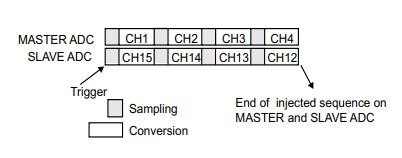
\includegraphics[width=0.75\textwidth]{adctimingmulti}
\caption{Timing diagram for MultiMode ADC conversions \cite{stmdatasheet}}
\label{fig:adctimingmulti}
\end{figure}

Since MultiMode uses two ADCs running simultaneously (with a 1.5 cycle delay), the maximum theoretical sampling rate for the primary ADC is approximately 1.15MHz. In practice, 851.4kHz was the maximum possible sampling rate - anything above this rate produced incomplete conversions for the final two channels.

After conversion, the ADC readings must be saved in a data buffer. Manually writing them to the buffer would significantly impact the maximum allowed sampling rate, so direct memory access (DMA) is used. A DMA stream is configured to write the ADC conversions to a memory buffer; however, using MultiMode requires special handling of these conversions. In normal modes, the 12-bit ADC conversions are stored as \verb|uint16_t| values. MultiMode saves simultaneous readings as \verb|uint32_t| values, with the first conversion (ADC1) stored in the first 16 bits of the \verb|uint32_t| value and the second (ADC2) stored in the last 16 bits of the \verb|uint32_t| value. Two macros were created to extract the individual ADC readings from these values. The code snippet below shows these two macros, as well as the initialization sequence for the ADCs in the initialization state.

\begin{lstlisting}[language=C++]
#define adc1conv(data) ((data) & 0xFFFF)
#define adc2conv(data) ((data >> 16) & 0xFFFF)
...
// start DMA from ADCs, writing TRIG_BUF_LEN samples to trig_buf (triggering state)
HAL_ADC_Start(&hadc2);
HAL_ADCEx_MultiModeStart_DMA(&hadc1, (uint32_t*)trig_buf, TRIG_BUF_LEN * NUM_MIC / 2);
// start timer that controls ADCs
HAL_TIM_Base_Start_IT(&htim3);
\end{lstlisting}

\subsection{Triggering State} \label{ssec:3s7s3}
The triggering state is used to decide if an acoustic pulse is incoming. In this state, the ADC records 64 samples from each microphone at 851.4kHz and saves their values to the buffer \verb|trig_buf|. Once the ADC conversion is finished and all readings are saved to the buffer, the recordings from each individual microphone are extracted from the buffer and the mean of each signal is calculated.

\begin{lstlisting}[language=C++]
float mic0_mean = 0, mic1_mean = 0, mic2_mean = 0, mic3_mean = 0;
for (int i = 0; i < TRIG_BUF_LEN * NUM_MIC/2; i += NUM_MIC/2) {
	mic0_mean += (float)adc1conv(trig_buf[i]);
	mic1_mean += (float)adc2conv(trig_buf[i]);
	mic2_mean += (float)adc1conv(trig_buf[i+1]);
	mic3_mean += (float)adc2conv(trig_buf[i+1]);
}
mic0_mean /= (float)TRIG_BUF_LEN;
mic1_mean /= (float)TRIG_BUF_LEN;
mic2_mean /= (float)TRIG_BUF_LEN;
mic3_mean /= (float)TRIG_BUF_LEN;
\end{lstlisting}

Next, the program checks if any of the microphones have recorded signals with sufficient variance. If any five subsequent values in a microphone’s signal exceed \verb|TRIG_THRES|, then that microphone has registered a significant signal. The code loops through every set of five values in each microphone’s signal and determines if any of the sets contain values all greater than \verb|TRIG_THRES|. If they do, then the flag \verb|exceedsThresholdmicN| is set to 1 for that microphone. This provides a robust method for determining when to record a full signal. For a 40kHz wave sampled at 851.4kHz, there are approximately 21 samples per full waveform; checking for five samples in a row detects the peaks of these waveforms when recording only a small number of samples.

\begin{lstlisting}[language=C++]
#define NUM_THRES_ROW 5
...
int exceedsThresholdmic0 = 0;
int exceedsThresholdmic1 = 0;
int exceedsThresholdmic2 = 0;
int exceedsThresholdmic3 = 0;
int loopLen = TRIG_BUF_LEN - NUM_THRES_ROW;
for (int i = 0; i < loopLen; i += 1) {
	int thres_count_mic0 = 0;
	int thres_count_mic1 = 0;
	int thres_count_mic2 = 0;
	int thres_count_mic3 = 0;
	
	// check if the next NUM_THRES_ROWS values exceed TRIG_THRES
	for (int t = 0; t < NUM_THRES_ROW; t++) {
		thres_count_mic0 += fabsf((float)adc1conv(trig_buf[i*NUM_MIC/2 + t*NUM_MIC/2 + 0]) - mic0_mean) > TRIG_THRES;
		thres_count_mic1 += fabsf((float)adc2conv(trig_buf[i*NUM_MIC/2 + t*NUM_MIC/2 + 0]) - mic1_mean) > TRIG_THRES;
		thres_count_mic2 += fabsf((float)adc1conv(trig_buf[i*NUM_MIC/2 + t*NUM_MIC/2 + 1]) - mic2_mean) > TRIG_THRES;
		thres_count_mic3 += fabsf((float)adc2conv(trig_buf[i*NUM_MIC/2 + t*NUM_MIC/2 + 1]) - mic3_mean) > TRIG_THRES;
	}
	
	if (thres_count_mic0 == NUM_THRES_ROW) exceedsThresholdmic0 = 1;
	if (thres_count_mic1 == NUM_THRES_ROW) exceedsThresholdmic1 = 1;
	if (thres_count_mic2 == NUM_THRES_ROW) exceedsThresholdmic2 = 1;
	if (thres_count_mic3 == NUM_THRES_ROW) exceedsThresholdmic3 = 1;
	
	// If all mics have been exceeded, we can break the loop
	if (exceedsThresholdmic0 && exceedsThresholdmic1 && exceedsThresholdmic2 && exceedsThresholdmic3) {
		break;
	}
}
\end{lstlisting}

After this, the total number of microphone signals that met the threshold criteria is summed. If more than one microphone met the threshold criteria, then the system transitions to the full recording state. Otherwise, the triggering state restarts and the above process repeats. In this state, each microphone has an associated LED for debugging; if the LED for a microphone lights up, then that microphone’s signal exceeded the threshold. This was crucial for ensuring the transmitter was pointing directly at the acoustic array during the data collection in Chapter \ref{chap:6c}.

\begin{lstlisting}[language=C++]
int exceedsThreshold = exceedsThresholdmic0 + exceedsThresholdmic1 + exceedsThresholdmic2 + exceedsThresholdmic3;

// if at least two microphones exceeded the threshold, move to the full recording state
if (exceedsThreshold > 1) {
	state = 2;                // transition to full recording state
	recording = 1;            // prevent interrupting ADC recording
	HAL_ADC_Start(&hadc2);    // start the secondary ADC
	HAL_ADCEx_MultiModeStart_DMA(&hadc1, (uint32_t*)adc_buf, ADC_BUF_LEN * NUM_MIC / 2); // start the primary ADC in DMA mode
	
	// otherwise, restart the triggering process
} else {
	HAL_ADC_Start(&hadc2);    // start the secondary ADC
	HAL_ADCEx_MultiModeStart_DMA(&hadc1, (uint32_t*)trig_buf, TRIG_BUF_LEN * NUM_MIC / 2); // start the primary ADC in DMA mode
}
\end{lstlisting}

\subsection{Full Recording and Recording Validation State} \label{ssec:3s7s4}
Not much happens during the full recording state besides ADC conversions. In this state, the STM32 halts reading from the IMU and updating the Madgwick filter. Even though the ADC conversions happen in the background and are written to a memory buffer using DMA, it is imperative that the ADC sampling occurs at the maximum sampling rate, so any potential sources of noise or resource use are halted.

Once the ADC conversion is finished and 2048 samples are recorded from each microphone, the system transitions to the recording validation state. This state is similar to the triggering state: its objective is to determine if the recording has enough variance to accurately perform a time shift calculation. Unlike the triggering state, a different method is used for determining the quality of the signal. The vast length of the full recording signals means that the standard deviation can be used as a good metric for the signal variance; it is assumed, due to the filtering of non-40kHz signals and amplification of 40kHz signals, that a signal with a sufficiently-large standard deviation contains the acoustic pulse from the transmitter. This was verified experimentally during testing in Chapter \ref{chap:6c}.

First, the mean and standard deviation of each signal is calculated. If the standard deviation of all four signals exceeds \verb|TRIG_THRES| and the IMU has been initialized, then the recording is considered sufficient for further data processing and the system transitions to the data processing state. If any of the signals fails to exceed the threshold, then the system returns to the triggering state; if this is the case, then the ADC buffers are reset. 

\begin{lstlisting}[language=C++]
// set recording flag to 0 because the ADC has stopped recording
recording = 0;

// stop the ADC trigger timer
HAL_TIM_Base_Stop_IT(&htim3);

// variables for calculating average and standard deviation for each microphone
mic0_avg = 0, mic1_avg = 0, mic2_avg = 0, mic3_avg = 0;
mic0_var = 0, mic1_var = 0, mic2_var = 0, mic3_var = 0;
mic0_stdev = 0, mic1_stdev = 0, mic2_stdev = 0, mic3_stdev = 0;

// calculate average of each mic signal
for (int i = 0; i < ADC_BUF_LEN * NUM_MIC / 2; i += NUM_MIC / 2) {
	mic0_avg += (float)adc1conv(adc_buf[i]);
	mic1_avg += (float)adc1conv(adc_buf[i+1]);
	mic2_avg += (float)adc2conv(adc_buf[i]);
	mic3_avg += (float)adc2conv(adc_buf[i+1]);
}
mic0_avg /= (float)ADC_BUF_LEN;
mic1_avg /= (float)ADC_BUF_LEN;
mic2_avg /= (float)ADC_BUF_LEN;
mic3_avg /= (float)ADC_BUF_LEN;

// calculate variance of each mic
for (int i = 0; i < ADC_BUF_LEN * NUM_MIC / 2; i += NUM_MIC / 2) {
	mic0_var += powf((float)adc1conv(adc_buf[i]) - mic0_avg, 2);
	mic1_var += powf((float)adc1conv(adc_buf[i+1]) - mic1_avg, 2);
	mic2_var += powf((float)adc2conv(adc_buf[i]) - mic2_avg, 2);
	mic3_var += powf((float)adc2conv(adc_buf[i+1]) - mic3_avg, 2);
}
mic0_var /= (float)(ADC_BUF_LEN - 1);
mic1_var /= (float)(ADC_BUF_LEN - 1);
mic2_var /= (float)(ADC_BUF_LEN - 1);
mic3_var /= (float)(ADC_BUF_LEN - 1);

// calculate standard deviation of each mic
mic0_stdev = sqrtf(mic0_var);
mic1_stdev = sqrtf(mic1_var);
mic2_stdev = sqrtf(mic2_var);
mic3_stdev = sqrtf(mic3_var);

// check if each microphone exceeds the threshold for "good" data
int stdev_above_thres = 0;
stdev_above_thres += mic0_stdev > (TRIG_THRES);
stdev_above_thres += mic1_stdev > (TRIG_THRES);
stdev_above_thres += mic2_stdev > (TRIG_THRES);
stdev_above_thres += mic3_stdev > (TRIG_THRES);

// if the signal is good and the initial IMU angle has been set (remove yaw), then
// move to the data processing state
if ((stdev_above_thres >= NUM_MIC) && imu_init_set){
	state = 4;
}
else{
	// reset all ADC buffers
	memset(adc_buf, 0, sizeof(adc_buf));
	memset(trig_buf, 0, sizeof(trig_buf));
	...
	// return to the trigger state
	state = 1;
	
	// restart the DMA from ADCs and the timer that controls the ADCs
	HAL_ADC_Start(&hadc2);
	HAL_ADCEx_MultiModeStart_DMA(&hadc1, (uint32_t*)trig_buf, TRIG_BUF_LEN * NUM_MIC / 2);
	HAL_TIM_Base_Start_IT(&htim3);
}
\end{lstlisting}

Figure \ref{fig:oscope4} shows an acoustic pulse recorded from four microphones on a Keysight oscilloscope. Figure \ref{fig:adc4} shows an acoustic pulse (with a slightly different receiver orientation) recorded using the STM32 and ADCs. In that figure, the ADC readings have been normalized, as described in Section \ref{ssec:3s8s2}. The ADC readings tend to be slightly noisier than the oscilloscope readings, but are sufficient for calculating time shifts.

\begin{figure}[htbp]
\centering
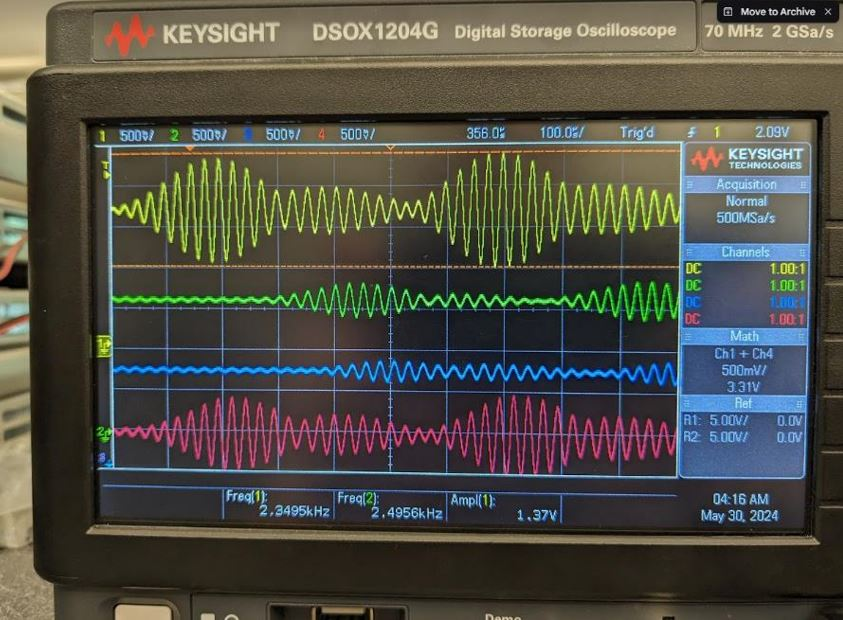
\includegraphics[width=0.75\textwidth]{oscope4}
\caption{Microphone recordings on Keysight oscilloscope}
\label{fig:oscope4}
\end{figure}

\begin{figure}[htbp]
\centering
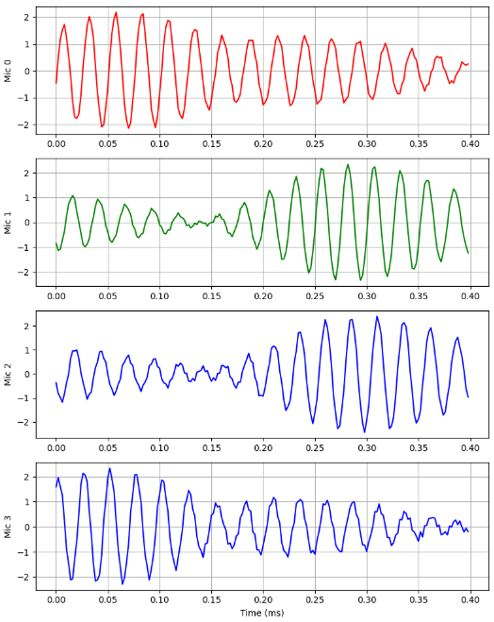
\includegraphics[width=0.75\textwidth]{adc4}
\caption{Microphone recordings on STM32 ADCs, slightly different receiver orientation}
\label{fig:adc4}
\end{figure}

\section{Calculating Time Shift} \label{sec:3s8}
Once a pulse has been recorded from all four microphones, the time shift between microphone recordings is calculated. Cross-correlations are a standard method for computing the time shift between two similar signals, but this method can be quite computationally-taxing  for large signals; for this reason, the fast Fourier transform (FFT) cross-correlation method is used. This takes the computation time from \(O(n^2)\) time to \(O(n \times log(n))\) time \cite{dspguide}. This section describes the theory of the FFT cross-correlation, then shows its implementation on the microcontroller.

\subsection{FFT Cross-Correlation Theory} \label{ssec:3s8s1}
Before the FFT cross-correlation can be understood, the basics of the convolution operation must be discussed. Cross-correlation and convolution are effectively the same operation, but with one of the signals flipped horizontally.

The convolution is a mathematical operation that takes two signals and produces a third signal \cite{dspguide}. The mathematical notation for a convolution of discrete signals is:

\begin{equation} \label{eq:3eq1}
x[n] * h[n] = y[n]
\end{equation}

Figure \ref{fig:convxn} shows an example convolution, while Figure \ref{fig:convexp} shows the components that make up the output of the convolution. A convolution operation can be thought of as flipping the second signal horizontally and then sliding it over the first signal, summing the area underneath the combination of both signals. Figure \ref{fig:convandcross} gives a wonderful visualization of the process, and the \href{https://en.wikipedia.org/wiki/Cross-correlation#/media/File:Cross_correlation_animation.gif}{GIF on the Wikipedia page for cross-correlation} is a fantastic animation showing how the cross-correlation of two signals is computed. 

\begin{figure}[htbp]
	\centering
	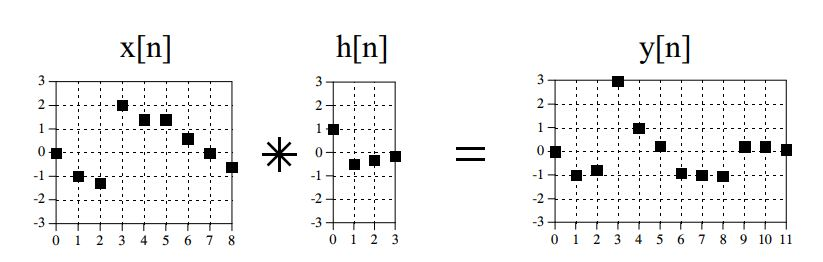
\includegraphics[width=.85\textwidth]{convxn}
	\caption{Convolution operation for two discrete signals \cite{dspguide}}
	\label{fig:convxn}
\end{figure}

\begin{figure}[htbp]
	\centering
	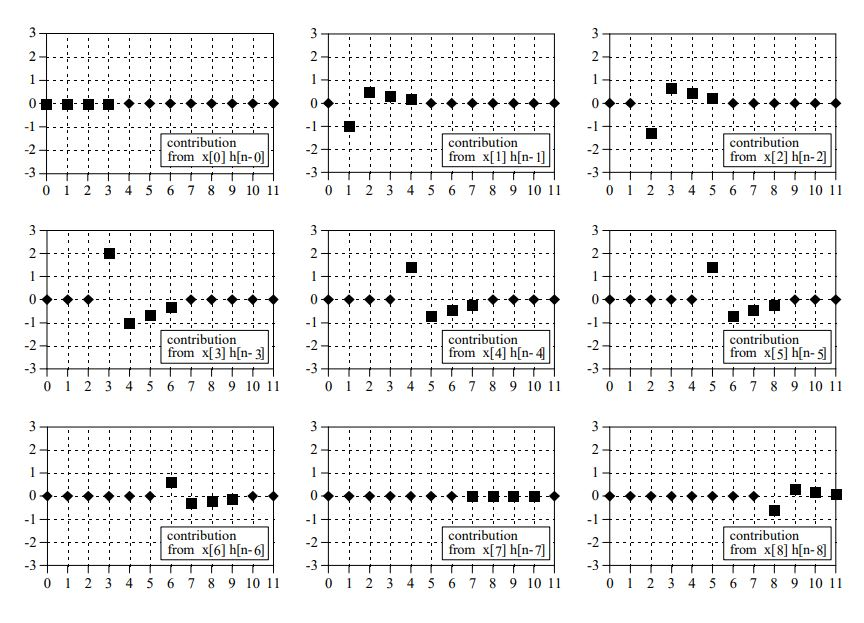
\includegraphics[width=.95\textwidth]{convexp}
	\caption{Convolution operation for two discrete signals, step-by-step process \cite{dspguide}}
	\label{fig:convexp}
\end{figure}

\begin{figure}[htbp]
	\centering
	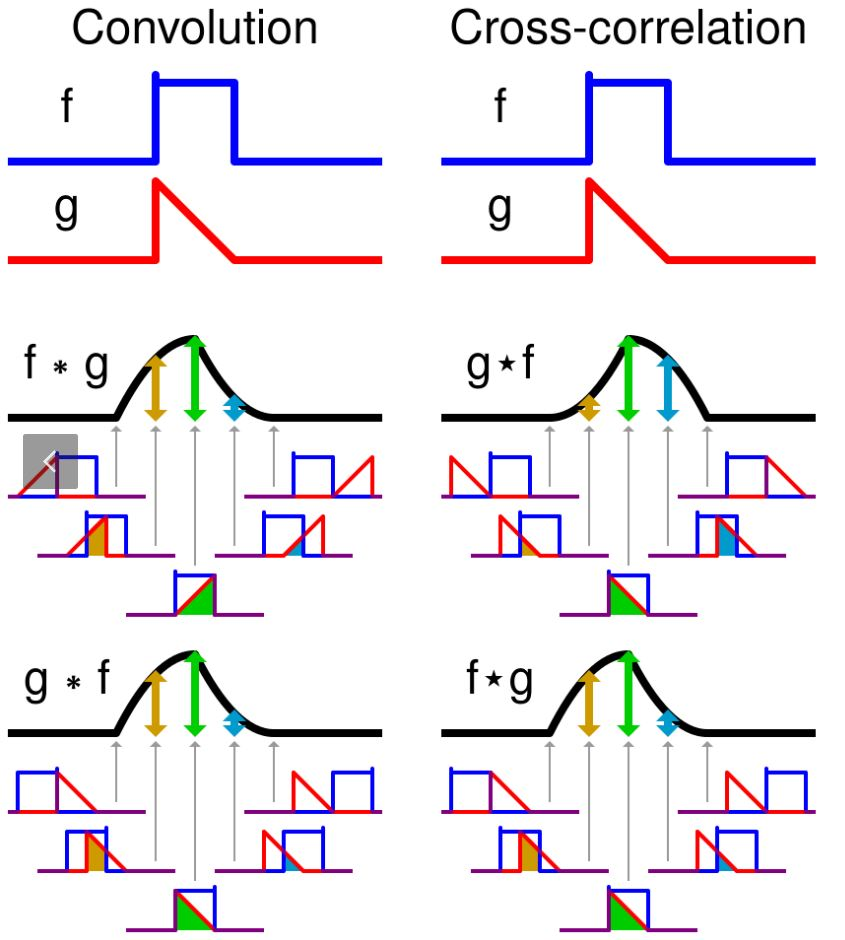
\includegraphics[width=0.65\textwidth]{convandcross}
	\caption{Convolution and cross-correlation operation for continuous signals \cite{wikicross}}
	\label{fig:convandcross}
\end{figure}

The convolution operation can be used to find the time shift between two similar signals. By first flipping the second signal horizontally (to negate the flip from the convolution operation), the two signals can be convolved to effectively slide them over each other. This process of flipping the second signal prior to the convolution is called "cross-correlation." In the output of the cross-correlation, the largest positive value corresponds to the shift between the signals \cite{dspguide}. This should make sense graphically; when the two signals fully overlap, the peaks of both align and the area under the curve shared between the signals is at a maximum. Figure \ref{fig:crosscorrex} shows this for two triangular pulses, with the shift between the two being correctly estimated as -0.5 (signal 2 lags signal 1 by 0.5 time units).

\begin{figure}[htbp]
	\centering
	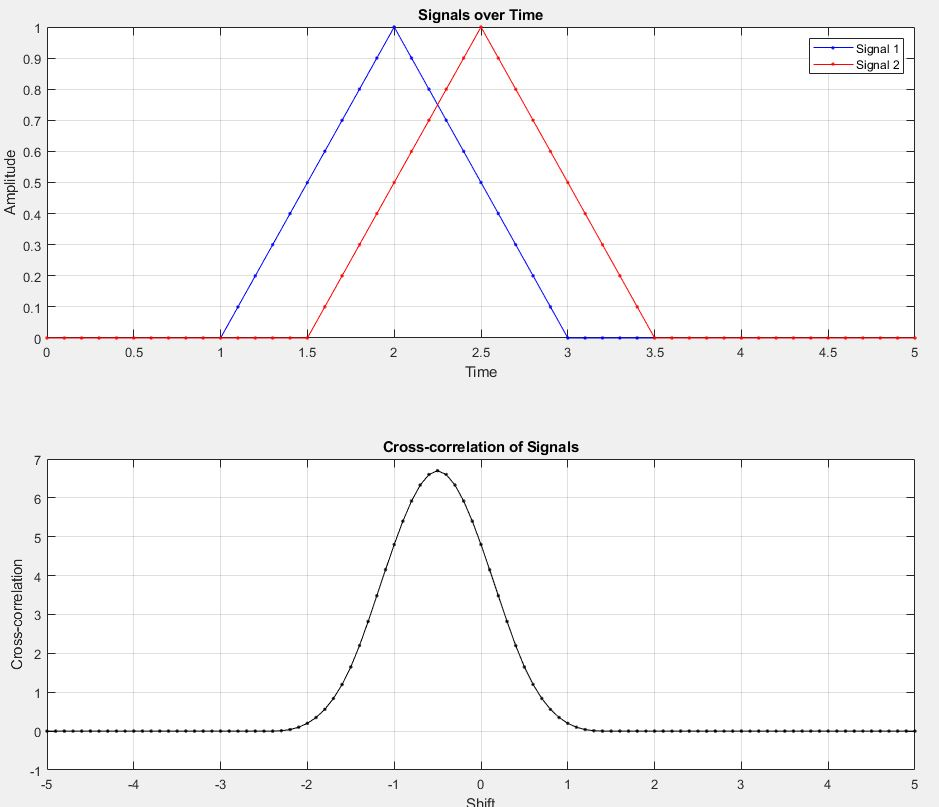
\includegraphics[width=.90\textwidth]{crosscorrex}
	\caption{Cross-correlation of two triangular pulses}
	\label{fig:crosscorrex}
\end{figure}

When computing the convolution, it is important to add “padding zeros” to the end of both signals. Without this step, the convolution operation is unable to fully “slide” the two signals over each other; it would instead wrap around to the beginning of the signal to complete the operation, which would give an incorrect result. For two signals of equal length \(n\), a total of \(n\) padded zeros should be added to each signal \cite{dspguide}.

The standard convolution operation is very computationally-expensive for long signals, with a convolution of two signals of equal length \(n\) taking \(O(n^2)\) time. However, convolution in the time domain corresponds to multiplication in the frequency domain, which is a much more efficient operation \cite{dspguide}. This changes the computation time for those same signals to \(O(n \times log(n))\) time. For signals of length 4096 (as this implementation uses, more details in next subsection), moving the operation to the frequency domain decreases the number of arithmetic operations required by approximately 99.9\%!

The name of this operation is the FFT convolution, or high-speed convolution. Figure \ref{fig:fftconvtheory} shows a graphical explanation for the operation. Both signals are converted from the time domain to the frequency domain using the FFT operation, multiplied in the frequency domain, and then the product is converted back to the time domain using the inverse FFT operation. For more details on the FFT and inverse FFT, see Chapter 12 of \textit{The Scientist and Engineer’s Guide to Digital Signal Processing} \cite{dspguide}. 

\begin{figure}[htbp]
\centering
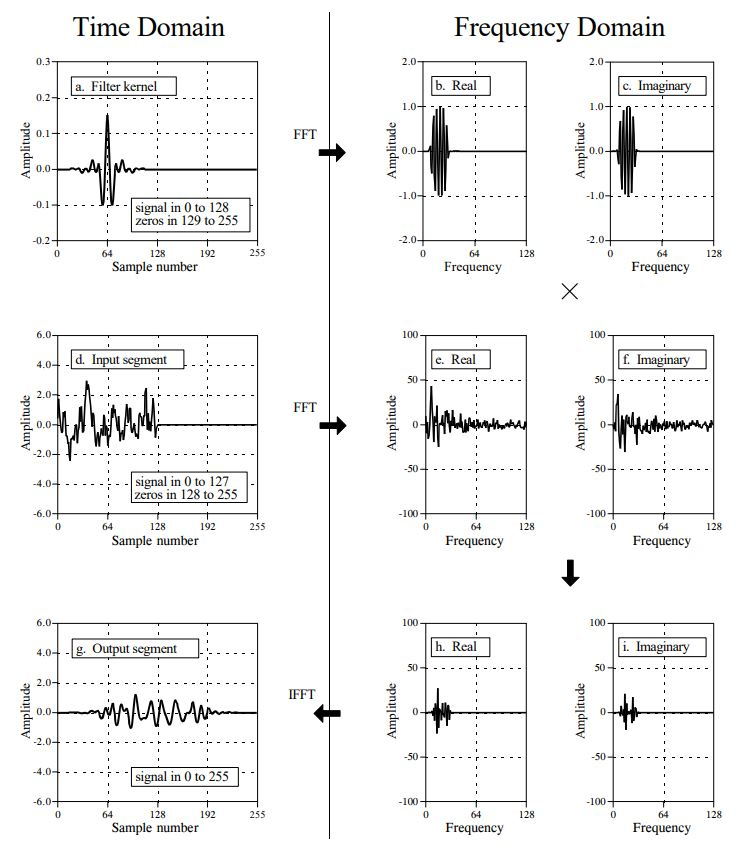
\includegraphics[width=0.9\textwidth]{fftconvtheory}
\caption{FFT convolution visual guide \cite{dspguide}}
\label{fig:fftconvtheory}
\end{figure}

Complex multiplication is required for the frequency domain; signals in that domain have both a real and imaginary component. Complex multiplication is carried out as shown below \cite{dspguide}:

\begin{equation} \label{eq:3eq2}
(a + bj) (c + dj) = (ac - bd) + j(bc + ad)
\end{equation}

\pagebreak

Finally, to perform FFT cross-correlation instead of FFT convolution, two approaches can be taken. First, the second signal can be flipped horizontally. Second, the complex conjugate of the second signal’s FFT transform can be taken. These operations are equivalent; one is in the time domain, and one is in the frequency domain. For this implementation, the complex conjugate operation is chosen, and its definition can be seen below \cite{dspguide}:

\begin{equation} \label{eq:3eq3}
conj(a + bj) = (a - bj)
\end{equation}

\subsection{FFT Cross-Correlation Implementation} \label{ssec:3s8s2}
The STM32 implementation makes heavy use of the \verb|arm_math.h| digital signal processing library \cite{arm}. This library implements all of the operations described in the previous section and many more. It is written for ARM Cortex M0, M3, M4, and M7 cores; the STM32H723ZG uses a Cortex M7 core. This subsection will walk through the code implementation of the FFT cross-correlation, which is used in the function \verb|calculate_time_shift()|.

Once the system transitions to the data processing state, the first step is to normalize the signals from each of the four microphones. Then, the function \verb|calculate_time_shift()| is run on each unique pair of microphone signals; all signals are compared to microphone 0 for simplicity. In future implementations, designing the program to compare the signals to the “best” signal (highest standard deviation, least noise) would be ideal.

\begin{lstlisting}[language=C++]
// buffers for holding normalized microphone buffers
float32_t mic0_buf[ADC_BUF_LEN];
float32_t mic1_buf[ADC_BUF_LEN];
float32_t mic2_buf[ADC_BUF_LEN];
float32_t mic3_buf[ADC_BUF_LEN];

// de-interleave the ADC values and normalize the data
int index = 0;
for (int i = 0; i < ADC_BUF_LEN * NUM_MIC / 2; i += NUM_MIC / 2) {
	mic0_buf[index] = (((float)adc1conv(adc_buf[i]) - mic0_avg) / mic0_stdev);
	mic1_buf[index] = (((float)adc1conv(adc_buf[i+1]) - mic1_avg) / mic1_stdev);
	mic2_buf[index] = (((float)adc2conv(adc_buf[i]) - mic2_avg) / mic2_stdev);
	mic3_buf[index] = (((float)adc2conv(adc_buf[i+1]) - mic3_avg) / mic3_stdev);
	index += 1;
}

// calculate time-shifts between mic0 and all other microphones
measured_time_shifts[0] = calculate_time_shift(mic0_buf,mic1_buf);
measured_time_shifts[1] = calculate_time_shift(mic0_buf,mic2_buf);
measured_time_shifts[2] = calculate_time_shift(mic0_buf,mic3_buf);
\end{lstlisting}

\pagebreak

Separately, a handler for the FFT operations used in \verb|arm_math.h| is initialized in the initialization state of the program. This handler defines the length of buffers used in these operations and must be a power of two. More details for the initialization can be found in the \verb|arm_math.h| documentation \cite{arm}.

\begin{lstlisting}[language=C++]
arm_rfft_fast_init_f32(&fftHandler, FFT_BUF_LEN);
\end{lstlisting}

The time shift function takes in pointers to two data buffers as inputs. These buffers contain the normalized data from two microphone signals. First, the microphone signals are moved into temporary buffers; padded zeros equal to the length of each signal are added. Then, the real FFT of each signal is computed (since both signals only contain real values, not complex). For memory efficiency, some buffers are reused.

\begin{lstlisting}[language=C++]
#define ADC_BUF_LEN 2048
#define FFT_BUF_LEN ADC_BUF_LEN*2
...
float32_t calculate_time_shift(float32_t *micA_buf, float32_t *micB_buf) {
	// load buffers
	float32_t fftBufIn[FFT_BUF_LEN];    /**< input to FFT */
	float32_t fftBuf1Out[FFT_BUF_LEN];  /**< output of first FFT */
	float32_t fftBuf2Out[FFT_BUF_LEN];  /**< output of second FFT */
	float32_t ifftBufIn[FFT_BUF_LEN];   /**< input to inverse FFT */
	float32_t ifftRealOut[FFT_BUF_LEN]; /**< output of inv FFT */
	
	// reset buffers to 0
	memset(fftBufIn, 0, sizeof(fftBufIn));
	memset(fftBuf1Out, 0, sizeof(fftBuf1Out));
	memset(fftBuf2Out, 0, sizeof(fftBuf2Out));
	memset(ifftBufIn, 0, sizeof(ifftBufIn));
	memset(ifftRealOut, 0, sizeof(ifftRealOut));
	
	// load micA values into fftBufIn (remaining values zeros for zero-padding)
	memcpy(fftBufIn, micA_buf, ADC_BUF_LEN * sizeof(float32_t));
	
	// perform real fft on zero-padded micA values
	arm_rfft_fast_f32(&fftHandler, fftBufIn, fftBuf1Out, 0);
	
	// reset fftBufIn
	memset(fftBufIn, 0, sizeof(fftBufIn));
	
	// load micB values into fftBufIn (remaining values zeros for zero-padding)
	memcpy(fftBufIn, micB_buf, ADC_BUF_LEN * sizeof(float32_t));
	
	// perform real fft on zero-padded micB values, put result into temporary buf
	arm_rfft_fast_f32(&fftHandler, fftBufIn, ifftBufIn, 0);
\end{lstlisting}

Next, the complex conjugate of the second signal’s FFT is taken. The FFT of the first signal and the complex conjugate of the second’s FFT are then multiplied using complex multiplication. Finally, the inverse real FFT of the product is taken (to return only real values, not complex) and stored in a buffer.

\begin{lstlisting}[language=C++]
	// calculate complex conjugate of micB real fft output (required for cross-correlation)
	arm_cmplx_conj_f32(ifftBufIn, fftBuf2Out, FFT_BUF_LEN);
	
	// reset temporary buf
	memset(ifftBufIn, 0, sizeof(ifftBufIn));
	
	// complex multiplication of the two fft output bufs
	arm_cmplx_mult_cmplx_f32(fftBuf1Out, fftBuf2Out, ifftBufIn, FFT_BUF_LEN);
	
	// perform inverse real fft on multiplication result
	arm_rfft_fast_f32(&fftHandler, ifftBufIn, ifftRealOut, 1);
\end{lstlisting}

The results in the inverse FFT output buffer are the output of the FFT cross-correlation operation. To find the most likely time shift between the signals, the index of the largest positive value is found.

\begin{lstlisting}[language=C++]
	// find argmax(ifft_output) to find time shift between signals
	int maxIndex = 0;
	float32_t maxVal = 0.0f;
	for (int i = 0; i < FFT_BUF_LEN; i++) {
		float32_t curVal = (ifftRealOut[i]);
		if (curVal > maxVal) {
			maxVal = curVal;
			maxIndex = i;
		}
	}
\end{lstlisting}

The x-axis of the cross-correlation results are not straightforward to understand. Figure \ref{fig:matlabcc} shows how the \verb|arm_math.h| implementation outputs its cross-correlation result of two signals. Compare this to Figure \ref{fig:crosscorrex}, which shows the shift on the x-axis instead of the output index.

\begin{figure}[htbp]
	\centering
	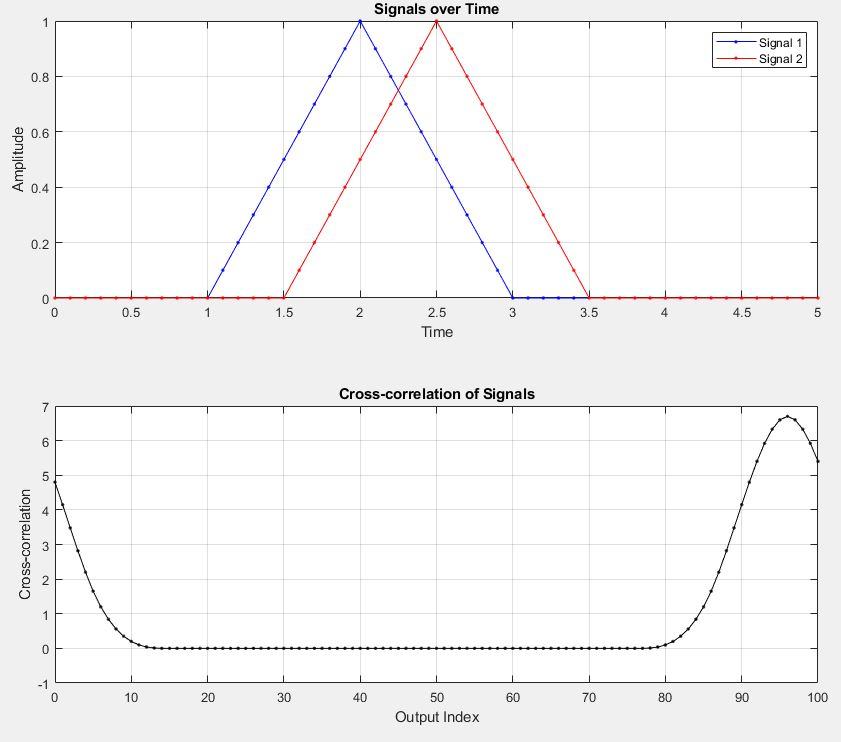
\includegraphics[width=0.9\textwidth]{matlabcc}
	\caption{Cross-correlation of two triangular pulses, STM32 implementation}
	\label{fig:matlabcc}
\end{figure}

To convert the maximum index of the output to a time shift, all values need to be shifted by half the number of output samples. Then, the index can be converted to a time shift in seconds using the sampling rate of the ADCs. The code below accomplishes this:

\begin{lstlisting}[language=C++]
	// shift is maxIndex if maxIndex < 0.5*fft_len, otherwise is maxIndex - fft_len
	float32_t adj_index = (maxI ndex < FFT_BUF_LEN/2) ? (float)(maxIndex) : (float)(-FFT_BUF_LEN + maxIndex);
	
	// convert shift index to seconds (275MHz / 323 ADC clock)
	float32_t shift = adj_index / (275000000 / 323);
\end{lstlisting}

Finally, the temporary buffers are reset, and the function returns \verb|shift|. All three shifts are stored in a list called \verb|measured_time_shifts[]|.

\pagebreak

\section{Acoustic Position Estimation} \label{sec:3s9}
After the time shifts between microphones have been calculated, the position of the receiver array’s center relative to the transmitter can be estimated. This section focuses on the position estimation workflow: rotating the microphones’ 3D positions by the current orientation of the array, running Hooke-Jeeves Search to get a relative position estimate, and incorporating the transmitter position to get the position estimate of the receiver array.

\subsection{Rotating the Microphone Array} \label{ssec:3s9s1}
The first step for position estimation is rotating the microphone array by its current orientation relative to the test frame. Section \ref{sec:4s4} covers the specifics of how that orientation is obtained; for this section, it is assumed that the IMU and Madgwick filter have initialized and the quaternion representation of the array’s orientation is available in floats \verb|q0, q1, q2,| and \verb|q3|. Section \ref{sec:4s4} also explains what a quaternion is; for brevity, it is an alternate way of expressing the rotation of one coordinate frame relative to another, whose elements fulfill the relationship in Equations \ref{eq:3eq4} and \ref{eq:3eq5}.

\begin{equation} \label{eq:3eq4}
	q = q_0 + iq_1 + jq_2 + kq_3
\end{equation}

\begin{equation} \label{eq:3eq5}
	i^2 = j^2 = k^2 = ijk = -1
\end{equation}

First, the initial yaw component of the orientation is removed from the current orientation estimate. This is covered in more detail in Section \ref{sec:6s1}, but for testing and data collection purposes, the position estimates are collected in a different coordinate frame than the global frame. The “global frame” refers to the NED (positive X points North, positive Y points East, positive Z points down) frame relative to the Earth’s magnetic and gravitational fields. For data collection, it was much easier to use the local frame of the Fo-SHIP: positive X points forward, positive Y points to the right, and positive Z points down. These are relative to the zero set point of the Fo-SHIP, which is on flat and level ground as measured by accelerometers. 

To convert the readings to the local frame of the Fo-SHIP (henceforth known as the “test frame”), the yaw component of the initial orientation estimate must be removed. This is achieved in three steps: creating a yaw-only quaternion, rotating the current orientation quaternion by the yaw-only quaternion, and normalizing the result.

\begin{lstlisting}[language=C++]
// extract the current orientation of the platform
// note: q0-3 are calculated in the Madgwick filter
Quaternion quat_raw = {q0, q1, q2, q3};

// create a quaternion to undo initial yaw rotation
Quaternion yaw_compensation = create_yaw_quaternion(init_yaw);

// apply the yaw compensation to the current quaternion
Quaternion quat = multiply_quaternions(yaw_compensation,quat_raw);

// normalize the result to ensure it's a valid rotation
normalize_quaternion(&quat);
\end{lstlisting}

The majority of the functions in this subsection are sourced from D. Rose’s article “Rotation Quaternions, and How to Use Them” \cite{quaternionuse}. The first function, \verb|create_yaw_quaternion()|, takes in an initial yaw in radians and forms a yaw-only quaternion. It is a partial version of a currently-unused function \verb|EulerAnglesToQuaternion()|, which is available in the code if needed. The initial yaw given in the code has already been negated during the IMU initialization, so this rotation represents the cancellation of the initial yaw.

\begin{lstlisting}[language=C++]
Quaternion create_yaw_quaternion(float yaw) {
	Quaternion q;
	q.w = cos(yaw / 2.0f);
	q.x = 0.0f;
	q.y = 0.0f;
	q.z = sin(yaw / 2.0f);
	return q;
}
\end{lstlisting}

Next, the two quaternions are multiplied. Multiplying quaternion A by quaternion B is the same as rotating a coordinate system by quaternion A first, followed by rotating it by quaternion B. For this implementation, it removes the initial yaw element. Quaternion multiplication is associative but non-commutative, so care must be taken in the order of the inputs. The multiplication function is derived in D. Rose’s article \cite{quaternionuse}.

\begin{lstlisting}[language=C++]
Quaternion multiply_quaternions(Quaternion q1, Quaternion q2) {
	Quaternion result;
	result.w = q1.w*q2.w - q1.x*q2.x - q1.y*q2.y - q1.z*q2.z;
	result.x = q1.w*q2.x + q1.x*q2.w + q1.y*q2.z - q1.z*q2.y;
	result.y = q1.w*q2.y - q1.x*q2.z + q1.y*q2.w + q1.z*q2.x;
	result.z = q1.w*q2.z + q1.x*q2.y - q1.y*q2.x + q1.z*q2.w;
	return result;
}
\end{lstlisting}

Lastly, the product is normalized. The multiplication of two quaternions should produce a quaternion that obeys Equations \ref{eq:3eq4} and \ref{eq:3eq5}, but floating point operations can cause small errors to accumulate. Normalization ensures that the quaternion is valid.

\begin{lstlisting}[language=C++]
void normalize_quaternion(Quaternion* q) {
	float magnitude = sqrt(q->w*q->w + q->x*q->x + q->y*q->y + q->z*q->z);
	q->w /= magnitude;
	q->x /= magnitude;
	q->y /= magnitude;
	q->z /= magnitude;
}
\end{lstlisting}

Now that the quaternion represents the orientation of the array relative to the test frame, the 3D coordinates of each microphone need to be rotated. The need for this operation is demonstrated graphically in Figure \ref{fig:anglecorr}. Without rotating the microphone array’s coordinates, the position estimate provided in the following subsections would only give the position of the transmitter normal to the face of the array! Ultimately, the position of the transmitter in the test frame is desired, so the orientation must be accounted for.

\begin{figure}[htbp]
	\centering
	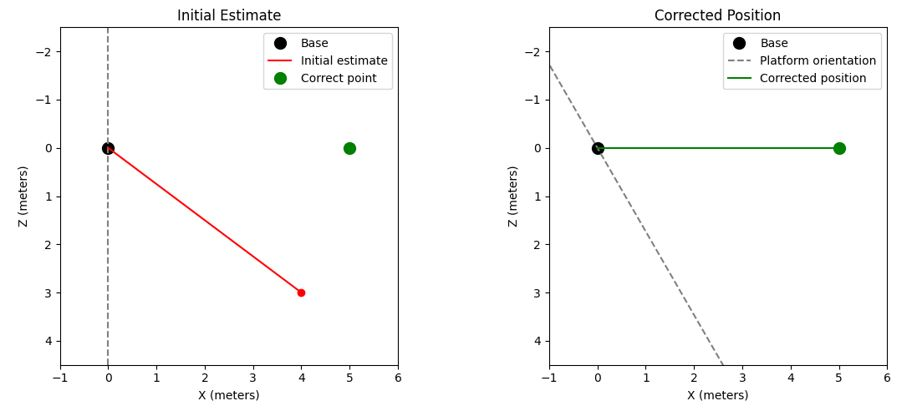
\includegraphics[width=\textwidth]{anglecorr}
	\caption{Orientation correction demonstration, 2D case}
	\label{fig:anglecorr}
\end{figure}

The 3D coordinate of each microphone’s center is stored in a custom struct, \verb|MicArray_t|. It makes use of another custom struct, \verb|Point3D|.
\begin{lstlisting}[language=C++]
typedef struct {
	float x, y, z;
} Point3D;

typedef struct {
	uint32_t num_mics;
	Point3D base_points[];  // Flexible array member
} MicArray_t;
\end{lstlisting}

In the initialization stage, the un-rotated \verb|MicArray_t| struct is formed. The system uses a coordinate system parallel to the test frame, and assumes that the center of the array is the origin (as opposed to the test frame, which uses the center of the Fo-SHIP's bottom platform as the origin).

\begin{lstlisting}[language=C++]
float32_t baseline = 0.250f
...
// initialize the mic array base points
MicArray_t* original_mic_array = createMicArray(NUM_MIC);
calculate_base_points(original_mic_array, baseline);
...
MicArray_t* createMicArray(uint32_t num_mics) {
	MicArray_t* mic_array = (MicArray_t*)malloc(sizeof(MicArray_t) + num_mics * sizeof(Point3D));
	if (mic_array != NULL) {
		mic_array->num_mics = num_mics;
	}
	return mic_array;
}
void calculate_base_points(MicArray_t* mic_array, float baseline) {
	// convert the baseline to a YZ spacing factor
	const float factor = baseline / 1.414f;
	
	// set coordinates for each microphone
	mic_array->base_points[0] = (Point3D){0.0f, -factor, -factor};
	mic_array->base_points[1] = (Point3D){0.0f, -factor,  factor};
	mic_array->base_points[2] = (Point3D){0.0f,  factor,  factor};
	mic_array->base_points[3] = (Point3D){0.0f,  factor, -factor};
	
	// if there are more than 4 microphones, set their coordinates to (0,0,0)
	// note: this implementation only uses 4, so this is just for error catching
	for (uint32_t i = 4; i < mic_array->num_mics; i++) {
		mic_array->base_points[i] = (Point3D){0.0f, 0.0f, 0.0f};
	}
}
\end{lstlisting}

Once in the data processing state, the original \verb|MicArray_t| is rotated by the yaw-compensated quaternion. Essentially, the function iterates through each 3D point in the \verb|MicArray_t|, and rotates it by the supplied quaternion.

\begin{lstlisting}[language=C++]
MicArray_t* rotated_mic_array = rotateMicArray(original_mic_array, quat);
...
MicArray_t* rotateMicArray(MicArray_t* original_mic_array, Quaternion quat) {
	if (original_mic_array == NULL) {
		return NULL;
	}
	
	MicArray_t* rotated_mic_array = createMicArray(original_mic_array->num_mics);
	if (rotated_mic_array == NULL) {
		return NULL;
	}
	
	
	for (uint32_t i = 0; i < original_mic_array->num_mics; i++) {
		rotated_mic_array->base_points[i] = rotatePoint(original_mic_array->base_points[i], quat);
	}
	
	return rotated_mic_array;
}
\end{lstlisting}

Rotating a point by a quaternion is quite similar to multiplying two quaternions together. The point, with coordinates \((X, Y, Z)\), is placed into its own quaternion \(v = 0 + iX + jY + kZ\). The point can be rotated by quaternion \(q\) by performing the multiplications in Equation \ref{eq:3eq6}, where \(q^{-1}\) is the inverse of the quaternion \cite{quaternionuse}.

\begin{equation} \label{eq:3eq6}
	v' = qvq^{-1}
\end{equation}

\begin{lstlisting}[language=C++]
Point3D rotatePoint(Point3D point, Quaternion q) {
	Point3D rotated;
	float x = point.x, y = point.y, z = point.z;
	
	// First multiplication: q * v
	float tw = -q.x*x - q.y*y - q.z*z;
	float tx =  q.w*x + q.y*z - q.z*y;
	float ty =  q.w*y - q.x*z + q.z*x;
	float tz =  q.w*z + q.x*y - q.y*x;
	
	// Second multiplication: (q * v) * q^-1
	// Note: for a unit quaternion, q^-1 = conjugate of q = (q.w, -q.x, -q.y, -q.z)
	rotated.x = tw*(-q.x) + tx*q.w + ty*(-q.z) - tz*(-q.y);
	rotated.y = tw*(-q.y) - tx*(-q.z) + ty*q.w + tz*(-q.x);
	rotated.z = tw*(-q.z) + tx*(-q.y) - ty*(-q.x) + tz*q.w;
	
	return rotated;
}
\end{lstlisting}

After these steps, the microphones will have been successfully rotated by the current orientation of the platform relative to the test frame, and the Hooke-Jeeves search algorithm can be run.

\subsection{Hooke-Jeeves Search} \label{ssec:3s9s2}
The majority of this part of the thesis implementation is based on the work from the Underwater Communication and Navigation Laboratory. Their GitHub repository, UCNLNav, contains a Matlab implementation of a variable-baseline time-difference-of-arrival acoustic position estimator \cite{ucnlnav}, which is precisely what this thesis is implementing. Significant modifications were made to their implementation, but their work forms the backbone of the acoustic position estimation system.

The Hooke-Jeeves search (HJS) algorithm is the keystone of the acoustic position estimation system. Also known as “pattern search,” it is an algorithm for finding the minimum of a function in an arbitrary number of dimensions \cite{hjsstan}. It was designed by Robert Hooke and T. A. Jeeves when they were working at Westinghouse Research Laboratories \cite{hjsog}. The most similar algorithm is gradient descent, an algorithm that finds the minimum of a function using information about the derivatives / gradient of the function. HJS is beneficial in that it does not require information about the gradient; this will be useful for future implementations where complex ocean acoustics models are incorporated into the sound propagation model and the gradient cannot be easily derived.

The HJS algorithm for \textbf{n} dimensions can be seen below in Algorithm \ref{alg:hooke-jeeves-3d}. A \href{https://en.wikipedia.org/wiki/Pattern\_search\_(optimization)\#/media/File:Direct\_search\_BROYDEN.gif}{GIF on the Wikipedia page for pattern search} provides a fantastic visualization of how HJS works. 

Essentially, the algorithm starts with an initial position estimate, an initial spacing, and a scaling factor. The algorithm requires some function that takes in a position in \textbf{n} dimensions and returns a scalar value. Along each dimension, points within ± one spacing unit of the initial position estimate are tested using the residual function. Whichever direction returns the smallest residual (or largest, if trying to maximize a function) is the new direction of motion. The algorithm will keep moving in that direction using a step size of one spacing unit until the residual function begins to increase. At that point, the spacing size is divided by the scaling factor (usually 2), and a new direction is chosen. This process repeats until a set number of iterations have taken place, the spacing size has reached some minimum threshold, or the residual has reached some minimum threshold \cite{hjsstan}. HJS and other pattern search methods are proven to converge \cite{hjsconv}, but may get stuck in local minima.

\begin{algorithm}
	\caption{Hooke-Jeeves Search Algorithm in \textbf{n} Dimensions} \label{alg:hooke-jeeves-3d}
	\begin{algorithmic}[1]
		\Require InitialPosition, MaxIterations, MinResidual, MinSpacing, ScaleFactor, InitialSpacing
		\Ensure OptimizedPosition
		
		\State $position \gets InitialPosition_{\mathbf{n} \times 1}$
		\State $newPosition \gets InitialPosition_{\mathbf{n} \times 1}$
		\State $residual \gets \infty$
		\State $spacing \gets InitialSpacing \times ScaleFactor$
		\State $iteration \gets 0$
		\State $newDirectionNeeded \gets false$
		\State $direction \gets \mathbf{0}_{\mathbf{n} \times 1}$
		
		\While{$iteration < MaxIterations$ \textbf{and} $residual > MinResidual$ \textbf{and} $spacing > MinSpacing$}
		\If{$newDirectionNeeded$}
		\State $spacing \gets spacing / ScaleFactor$
		\For{each dimension $\mathbf{d}$ in $\mathbf{n}$}
		\State $direction \gets \mathbf{0}_{\mathbf{n} \times 1}$
		\State $direction(\mathbf{d}) \gets 1$
		\State $testPosition \gets position + direction \times spacing$
		\State $residualList(2\mathbf{d}) \gets$ CalculateResidual($testPosition$)
		\State $testPosition \gets position - direction \times spacing$
		\State $residualList(2\mathbf{d}+1) \gets$ CalculateResidual($testPosition$)
		\EndFor
		\If{min$(residualList) < residual$}
		\State $direction \gets \arg\!\min_{direction}(residualList)$
		\State $residual \gets$ min$(residualList)$
		\State $position \gets position + direction \times spacing$
		\State $newDirectionNeeded \gets false$
		\Else
		\State $newDirectionNeeded \gets true$
		\EndIf
		\Else
		\State $prevResidual \gets residual$
		\State $newPosition \gets position + direction \times spacing$
		\State $residual \gets$ CalculateResidual($newPosition$)
		\If{$residual < prevResidual$}
		\State $position \gets newPosition$
		\Else
		\State $residual \gets prevResidual$
		\State $newDirectionNeeded \gets true$
		\EndIf
		\EndIf
		\State $iteration \gets iteration + 1$
		\EndWhile
		
		\Return $position$
	\end{algorithmic}
\end{algorithm}

For this implementation, two choices are considered: should a 2D or 3D HJS algorithm be run? While the position estimate and receiver positions exist in three dimensions, short baselines tend to cause issues when running 3D HJS. The UCNLNav Matlab implementation was tested with the baselines of the physical iSBL array and simulated results for a transmitter approximately 7 meters away. The original code runs 3D HJS but was modified to run HJS in 2D, with results locked to a single plane parallel to the XY plane. A small amount of noise was added to measurements in order to mimic real-world environments. 

Multiple planes, spaced 0.1m apart, were tested with the 2D HJS algorithm. Figure \ref{fig:3dhjsmat} shows the results of this testing. The star represents the true transmitter location, while the triangles represent the three best 2D HJS results, and the dots represent the HJS results for each plane. If the algorithm were able to determine the 3D position using the acoustic data alone, it would be expected that the three triangles would overlap at the star. However, the graph shows that this is not the case. In fact, 3D HJS was run in addition to the 2D test, and its position estimate is shown with the square.

The final residual of all planes between \(z = -2m\) and \(z = -10m\) were very close to one another, each within approximately 5\% of the lowest value.  It can be seen that all minimum points lie on the vector between the center of the receiver array and the true transmitter location. The 3D HJS algorithm has a difficult time determining where upon the vector the true location is, but the square does indeed lie upon the vector. It should be noted that the Matlab simulation in Figure \ref{fig:3dhjsmat} is flipped vertically from this thesis’s implementation.

\begin{figure}[htbp]
	\centering
	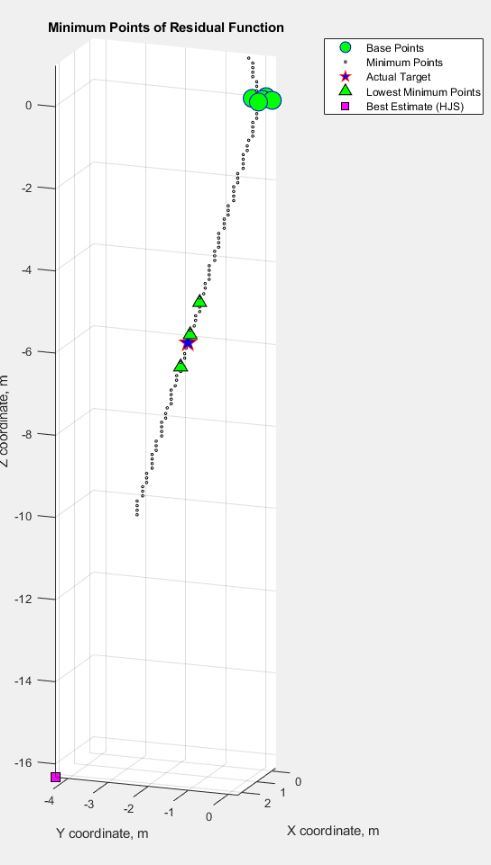
\includegraphics[width=0.85\textwidth]{3dhjsmat}
	\caption{Matlab HJS results, search run on each 2D plane}
	\label{fig:3dhjsmat}
\end{figure}

Thankfully, this system is designed for underwater use, and one particular sensor can make up for the short baseline’s shortcomings: a pressure (depth) sensor. These sensors measure the depth of an underwater vehicle by converting water pressure readings into depth measurements. Relatively inexpensive and commercially-available sensors such as Blue Robotics’ Bar30 pressure sensor are capable of accurate depth measurement within 2m at up to 300m deep \cite{blueps}. For the underwater implementation, the depth measurement can determine the z-coordinate of the transmitter, while the HJS algorithm determines the x- and y-coordinates.

\pagebreak

For the above-water implementation and testing, the HJS algorithm was run in 2D with a simulated depth measurement providing the depth coordinate. Since the testing is performed horizontally (see Section \ref{sec:6s1} for more details), the x-coordinate represents the depth of the above-water system. The measurement was simulated, since pressure sensors provide no position information in air; this was accomplished by combining the true x-coordinate of the transmitter with the true x-coordinate of the iSBL array and adding random noise. The true position of the transmitter is known prior to testing; in the full underwater implementation, the position would be given via GPS coordinates. The true x-coordinate of the iSBL array’s center is sent from the Fo-SHIP’s ESP32 to the iSBL array’s STM32 as described in Section \ref{ssec:2s5s3}. Both of these values are crucial for determining the true “depth” of the system.

The initial position estimate is set with the depth measurement as the initial x-coordinate, and with zeros for the y- and z-coordinates. Then, the 2D HJS function is called. It takes in the 3D coordinates of each rotated microphone (see Section \ref{ssec:3s9s1}), the initial position estimate, the measured time shifts from each microphone (see Section \ref{ssec:3s8s2}), and the exit condition parameters below:

\begin{itemize}[noitemsep,topsep=0pt,]
	\item A maximum of 1000 iterations (generally only takes 60-70 iterations)
	\item A minimum residual of 1e-13 m$^2$ (generally returns with 1e-9 m$^2$)
	\item A minimum spacing of 1e-6 m (generally the condition that causes termination)
\end{itemize}

If any of the exit conditions are met, then the HJS terminates and returns its current position estimate. The parameters were determined experimentally; the minimum spacing tends to be the most important, as a spacing of below 0.001mm not providing much additional accuracy. In fact, this parameter could be raised higher without affecting the position estimation accuracy by much. For the full underwater implementation, these parameters would need to be re-tuned.

\begin{lstlisting}[language=C++]
// the true position of the transmitter in meters
float true_x = 3.880f;
float true_y = 0.0f;
float true_z = -0.682f;

// define an initial guess for the transmitter's XYZ position
// note: noise in the depth measurement is simulated here using randn()
Point3D init_pos_est;
init_pos_est.x = true_x - fossl_x + randn(0.0f, 0.005f);
init_pos_est.y = 0;
init_pos_est.z = 0;

// perform hooke-jeeves search to minimize the residual function
raw_isbl_pos_est = hooke_jeeves_search_2d(rotated_mic_array, init_pos_est, measured_time_shifts, 1000, 1e-13, 1e-6, 2.0f);
\end{lstlisting}

The STM32 implementation of 2D HJS can be seen below in its entirety. It follows Algorithm \ref{alg:hooke-jeeves-3d} very closely, testing different positions along the y- and z-axes.

\begin{lstlisting}[language=C++]
Point3D hooke_jeeves_search_2d(MicArray_t* mic_array, Point3D init_pos_est, float32_t measured_time_shifts[], int max_iter, float32_t min_residual, float32_t min_spacing, float32_t scale_factor) {
Point3D pos_est = init_pos_est;
Point3D new_pos_est = init_pos_est;
float32_t residual = 1e9; // meters^2
float32_t residual_arr[4];
float32_t prev_residual = 1e10;
float32_t spacing = 2; // meters
int new_dir_index = 0;
int new_dir_flag = 0;
int iter = 0;
int dy = 0;     /**< direction modifier for y-axis */
int dz = 0;     /**< direction modifier for z-axis */

while ((iter < max_iter) && (residual > min_residual) && (spacing > min_spacing)){
	
	// if previous move gave a worse residual, choose new direction
	if (new_dir_flag){
		
		// every time a new direction is chosen, spacing is reduced
		spacing /= scale_factor;
		
		// test plus/minus spacing in each dimension, save residuals
		int d_idx = 0;
		for (int dy_ = -1; dy_ <= 1; dy_ += 2){
			new_pos_est.y = pos_est.y + (dy_) * spacing;
			new_pos_est.z = pos_est.z;
			residual_arr[d_idx] = calculate_residual(mic_array, new_pos_est, measured_time_shifts);
			d_idx ++;
		}
		for (int dz_ = -1; dz_ <= 1; dz_ += 2){
			new_pos_est.y = pos_est.y;
			new_pos_est.z = pos_est.z + (dz_) * spacing;
			residual_arr[d_idx] = calculate_residual(mic_array, new_pos_est, measured_time_shifts);
			d_idx ++;
		}
		
		// find direction that gives smallest residual
		new_dir_index = arg_min(residual_arr, d_idx);
		
		// if that direction has a smaller residual than the previous residual, move in that direction
		if (residual_arr[new_dir_index] < residual){
			residual = residual_arr[new_dir_index];
			
			// determine what the new direction is
			if (new_dir_index < 2) {
				dy = (new_dir_index % 2) * 2 - 1;
				dz = 0;
			} else {
				dy = 0;
				dz = ((new_dir_index - 2) % 2) * 2 - 1;
			}
			
			// calculate new position based on that direction
			new_pos_est.y = pos_est.y + (dy) * spacing;
			new_pos_est.z = pos_est.z + (dz) * spacing;
			
			// save as new best position estimate
			pos_est = new_pos_est;
			
			// start moving in that direction until improvement stops
			new_dir_flag = 0;
		}
		
		// otherwise, repeat above process
		else{
			new_dir_flag = 1;
		}
	}
	
	// otherwise, continue in same direction
	else{
		// calculate residual for next position
		prev_residual = residual;
		new_pos_est.y = pos_est.y + (dy) * spacing;
		new_pos_est.z = pos_est.z + (dz) * spacing;
		residual = calculate_residual(mic_array, new_pos_est, measured_time_shifts);
		
		// if new residual is smaller than previous residual, keep moving in that direction
		if (residual < prev_residual){
			pos_est = new_pos_est;
		}
		
		// otherwise, choose a new direction on next iteration
		else{
			residual = prev_residual
			new_dir_flag = 1;
		}
	}
	
	iter++;
}

// once an exit condition has been satisfied, break the loop
return pos_est;
}
\end{lstlisting}

Given a 3D position estimate of the transmitter, the 3D positions of each microphone, and the measured time shifts as inputs, the residual function returns the sum of squared differences between the measured time shifts and the expected (calculated) time shifts for that position estimate. Essentially, the function determines what the time shifts would be if the transmitter was at the 3D position given as input; then, it compares these expected time shifts to the measured time shifts. If the position estimate given is at the true position of the transmitter (and assuming no noise or error), then the residual function will return zero. The further that the position estimate is from the true position of the transmitter, the larger the residual is. For four microphones, the residual function is smooth and has few local minima; most are very close to the global minimum. This makes it easy for the HJS to converge on a minimum near the true transmitter location.

The residual function, as well its helper functions, can be seen below. The sum of squared differences is used (as opposed to the absolute difference) because it makes the residual function steeper; it also helps avoid any single time difference from being too far off. 

The function \verb|calculate_toa()| uses the 3D coordinates of each rotated microphone and the test position to calculate the Euclidean distance between each microphone and the test point. Then, it converts the distance to a time-of-arrival measurement using the speed of sound for the acoustic medium (in this case, air). The residual function subtracts each time-of-arrival from the first microphone’s time-of-arrival to get the time differences. Lastly, it calculates the sum of squared differences between these estimated shifts and the measured time shifts using \verb|calculate_squared_diff()|, and returns the value to the HJS function.

\begin{lstlisting}[language=C++]
float32_t calculate_residual(MicArray_t* mic_array, Point3D target_point, float32_t measured_time_shifts[]) {
	float32_t toa0 = 0;   /**< time of arrival for first mic */
	float32_t toaN = 0;   /**< time of arrival for Nth mic */
	float32_t* target_time_shifts = malloc((mic_array->num_mics - 1) * sizeof(float32_t));
	
	toa0 = calculate_toa(mic_array->base_points[0], target_point, sound_speed_mps);
	
	// for each mic, calculate the time of arrival (TOA)
	for (int i = 1; i < mic_array->num_mics; i++) {
		toaN = calculate_toa(mic_array->base_points[i], target_point, sound_speed_mps);
		
		// time shift is the first mic TOA minus the Nth mic TOA
		target_time_shifts[i-1] = toa0 - toaN;
	}
	
	// take the sum of squared differences between the time shifts
	float32_t residual = calculate_squared_diff(measured_time_shifts, target_time_shifts, mic_array->num_mics - 1);
	
	// save the calculated time shifts into a global array (for debugging / comparing to the real estimates)
	for (int i = 0; i < mic_array->num_mics - 1; i++) {
		calcd_time_shifts[i] = target_time_shifts[i];
	}
	
	// free the target time shift memory to avoid memory leaks
	free(target_time_shifts);
	return residual;
}

float32_t calculate_toa(Point3D pointA, Point3D pointB, float32_t sound_speed_mps) {
	float32_t xA = pointA.x;
	float32_t yA = pointA.y;
	float32_t zA = pointA.z;
	float32_t xB = pointB.x;
	float32_t yB = pointB.y;
	float32_t zB = pointB.z;
	float32_t euclidean_dist = sqrt((xA-xB)*(xA-xB) + (yA-yB)*(yA-yB) + (zA-zB)*(zA-zB));
	float32_t toa = euclidean_dist / sound_speed_mps;
	return toa;
}

float32_t calculate_squared_diff(float32_t measured_data[], float32_t target_data[], int data_len){
	float32_t squared_diff = 0;
	for (int i = 0; i < data_len; i++){
		squared_diff += ((measured_data[i] - target_data[i])*(measured_data[i] - target_data[i]));
	}
	return squared_diff;
}
\end{lstlisting}

Lastly, the \verb|arg_min()| function locates the index of the minimum value of the \verb|residual_arr[]| list. This step is crucial for determining the best direction in the HJS algorithm.

\begin{lstlisting}[language=C++]
int arg_min(float32_t data_array[], int data_len){
	float32_t minValue = 1e10;
	int minIndex = 0;
	for (int i = 0; i < data_len; i++) {
		if (data_array[i] < minValue) {
			minValue = data_array[i];
			minIndex = i;
		}
	}
	return minIndex;
}
\end{lstlisting}

\subsection{Incorporating Transmitter Position} \label{ssec:3s9s3}
Once an exit condition is met, the HJS function returns a position estimate to the main code. This estimate describes the position of the transmitter relative to the center of the receiver array. However, the transmitter position in the test frame is always known, using GPS coordinates in the full underwater implementation or measured 3D coordinates in this air-based implementation. These two measurements need to be combined.

Since the position estimate from the HJS algorithm gives the relative position of the transmitter from the iSBL array’s center, the inverse of this vector describes the location of the receiver array relative to the transmitter. This inverse can be added to the transmitter’s true position to get the estimated position of the iSBL array in the test frame. For a one-dimensional example: if a receiver determines a transmitter is located 3 meters ahead of itself in the x-direction, and it knows that the transmitter is located at \verb|x=5m|, then the receiver must be located at \verb|x=2m|. The code below implements this on the STM32 using the 3D position estimates.

\begin{lstlisting}[language=C++]
float true_x = 3.880f;
float true_y = 0.0f;
float true_z = -0.682f;
...
// perform hooke-jeeves search to minimize the residual function
raw_isbl_pos_est = hooke_jeeves_search_2d(rotated_mic_array, init_pos_est, measured_time_shifts, 1000, 1e-13, 1e-6, 2.0f);
...
// subtract estimated position to transmitter from known transmitter location to get receiver position
raw_isbl_pos_est.x = true_x - raw_isbl_pos_est.x;
raw_isbl_pos_est.y = true_y - raw_isbl_pos_est.y;
raw_isbl_pos_est.z = true_z - raw_isbl_pos_est.z;
\end{lstlisting}

Finally, the acoustic position estimate for a single iteration is saved in the variable \verb|raw_isbl_pos_est[]|. From recording a single acoustic pulse on the four receivers, measuring the time shift between microphones, rotating the microphones’ 3D positions using the current orientation, running 2D HJS with the simulated depth measurement, and reflecting the position estimate across the transmitter, a single acoustic position estimate is formed! In Chapter \ref{chap:5c}, this position estimate is improved using Kalman filtering.

\bibliographystyle{IEEEtran}
\bibliography{../thesis}

\end{document}